\documentclass[degree=master,tocarialchapter]{thuthesis}
% 选项
%   degree=[bachelor|master|doctor|postdoctor], % 必选,学位类型
%   language=[chinese|english], % 可选(默认:chinese),论文的主要语言
%   secret,                % 可选(默认:关闭),是否有密级
%   tocarialchapter,       % 可选(默认:关闭),章目录中使用黑体(这项表示同时打开下面两项)
%   tocarialchapterentry,  % 可选(默认:关闭),单独控制章标题在目录中使用黑体
%   tocarialchapterpage,   % 可选(默认:关闭),单独控制章页码在目录中使用黑体

% 所有其它可能用到的包都统一放到这里了,可以根据自己的实际添加或者删除。
\usepackage{thuthesis}

% 定义所有的图片文件在 figures 子目录下
\graphicspath{{figures/}}

% 可以在这里修改配置文件中的定义。导言区可以使用中文。
% \def\myname{薛瑞尼}

\begin{document}

%%% 封面部分
\frontmatter
\thusetup{
  %******************************
  % 注意:
  %   1. 配置里面不要出现空行
  %   2. 不需要的配置信息可以删除
  %******************************
  %
  %=====
  % 秘级
  %=====
  secretlevel={秘密},
  secretyear={10},
  %
  %=========
  % 中文信息
  %=========
  ctitle={SDN中LDoS防御机制研究},
  cdegree={工程硕士},
  cdepartment={计算机科学与技术系},
  cmajor={计算机技术},
  cauthor={谢仁杰},
  csupervisor={徐明伟教授},
  % cassosupervisor={陈文光教授}, % 副指导老师
  % ccosupervisor={某某某教授}, % 联合指导老师
  % 日期自动使用当前时间,若需指定按如下方式修改:
  % cdate={超新星纪元},
  %
  % 博士后专有部分
  catalognumber     = {分类号},  % 可以留空
  udc               = {UDC},  % 可以留空
  id                = {编号},  % 可以留空: id={},
  cfirstdiscipline  = {计算机科学与技术},  % 流动站(一级学科)名称
  cseconddiscipline = {系统结构},  % 专 业(二级学科)名称
  postdoctordate    = {2009 年 7 月——2011 年 7 月},  % 工作完成日期
  postdocstartdate  = {2009 年 7 月 1 日},  % 研究工作起始时间
  postdocenddate    = {2011 年 7 月 1 日},  % 研究工作期满时间
  %
  %=========
  % 英文信息
  %=========
  etitle={Research on defense of LDoS in SDN},
  % 这块比较复杂,需要分情况讨论:
  % 1. 学术型硕士
  %    edegree:必须为Master of Arts或Master of Science(注意大小写)
  %             “哲学、文学、历史学、法学、教育学、艺术学门类,公共管理学科
  %              填写Master of Arts,其它填写Master of Science”
  %    emajor:“获得一级学科授权的学科填写一级学科名称,其它填写二级学科名称”
  % 2. 专业型硕士
  %    edegree:“填写专业学位英文名称全称”
  %    emajor:“工程硕士填写工程领域,其它专业学位不填写此项”
  % 3. 学术型博士
  %    edegree:Doctor of Philosophy(注意大小写)
  %    emajor:“获得一级学科授权的学科填写一级学科名称,其它填写二级学科名称”
  % 4. 专业型博士
  %    edegree:“填写专业学位英文名称全称”
  %    emajor:不填写此项
  edegree={Master of Engineering},
  emajor={Computer Technology},
  eauthor={Xie Renjie},
  esupervisor={Professor Xu Mingwei},
  % eassosupervisor={Chen Wenguang},
  % 日期自动生成,若需指定按如下方式修改:
  % edate={December, 2005}
  %
  % 关键词用“英文逗号”分割
  ckeywords={SDN, LDoS, 防御},
  ekeywords={SDN, LDoS, defense}
}

% 定义中英文摘要和关键字
\begin{cabstract}
  LDoS(Low-rate Denial of Service)攻击作为一种特殊的DoS(Denial of Service)攻击,对互联网有极大的威胁。由于TCP(Transmission Control Protocol)协议的超时重传机制,LDoS攻击可以通过发送周期性的脉冲流引发TCP吞吐量明显的下降。LDoS攻击具有较低的平均速率,因而该攻击很难被检测和限制。

  近来,SDN(Software-Defined Networking)作为一种有潜力的新型网络范式,为DoS攻击的防御工作提供了新的方法。很多基于SDN的防御系统被提出来防御各种各样的DoS攻击。但是,这些方案都没有考虑LDoS攻击。

  本文提出了两种基于SDN的防御方案来有效的限制LDoS攻击:基于带宽保障的方案和基于动态周期性检测的方案。第一种方案首先在交换机的端口上安装特制的Meter规则。接下来,当有新的流进入网络的时候,控制器判断该流是否为TCP流。在新流不是TCP流的情况下,将该流的流表规则与Meter规则绑定。通过Meter规则限制非TCP流的聚合吞吐量,为TCP流保留带宽。这样,TCP流就不会进入超时重传状态,吞吐量可以保持在正常水平。第二种方案通过在交换机的端口上安装特制的流表规则来检测TCP流的聚合吞吐量是否有显著下降。接下来,它通过端口处统计的聚合吞吐量是否存在周期性来确认LDoS攻击。然后,通过平均欧式距离方法精准识别LDoS攻击流。最后,控制器通过在入口交换机处安装相应的限制规则来有效限制LDoS攻击。

  本文在Floodlight控制器上实现了两种方案。在真实SDN实验中,本文采用了单攻击源和分布式的LDoS攻击来测试方案的有效性。实验结果证明,两种方案都能够有效的防御LDoS攻击,而且只引入了极低的系统开销。最后,本文分析两种方案的适用场景。第一种方案适用于保护重要TCP流,但不适合与广泛部署。第二种方案可广泛部署在网络中以消除LDoS攻击对系统造成的影响。

\end{cabstract}

% 如果习惯关键字跟在摘要文字后面,可以用直接命令来设置,如下:
% \ckeywords{\TeX, \LaTeX, CJK, 模板, 论文}

\begin{eabstract}
  As a special Denial of Service (DoS) attack, the Low-rate Denial of Service (LDoS) attack is essentially a great threat to the Internet. Due to the Timeout retransmission mechanism, It causes significant throughput degradation of TCP flows by generating periodical pulsing flows. Due to its low rate, the attack is difficult to be detected and throttled.

  Recently, Software-Defined Networking (SDN) has emerged as a promising network paradigm. It provides new methods to defend against DoS attacks. Several SDN-based defense systems have been proposed to deal with various Denial of Service (DoS) attacks. However, they fail to consider the low-rate TCP attack.

  In this paper, Two SDN-based defense schemes are proposed to effectively throttle the LDoS attack. The first scheme is based on bandwidth reservation and the second scheme is based on dynamic periodical detection. The first scheme installs Meter rules in ports of switches. If a non-TCP flow enters the network, it will be associated with a meter rule for rate limiting. Through meter rules, the bandwidth is reserved for TCP flows. Thus, TCP flows will not be forced to retransmit and their aggregated throughput will remain normal. 


  The second scheme detects the attack by installing crafted flow rules to monitor the degradation of aggregated TCP throughput in ports of switches. It confirms the attack by judging whether there is periodicity for aggregated throughput, and accurately identifies attack flows with Mean Euclidean Distance. Identified attack flows will be effectively throttled by installing mitigation rules in ingress switches.

  Two schemes are implemented in the Floodlight controller. The LDoS attack generated by single and multiple sources is applied to evaluate the schemes.    Experiments in a real SDN testbed demonstrate their effectiveness for defending against the LDoS attack. Moreover, the schemes introduce a small overhead. Two schemes are suitable for different scenarios. The first scheme is suitable for protecting important flows. However, the wide deployment of the scheme brings a negative impact on other flows. The wide deployment of the second scheme helps to eliminate the influence of the attack.

\end{eabstract}

% \ekeywords{\TeX, \LaTeX, CJK, template, thesis}

% 如果使用授权说明扫描页,将可选参数中指定为扫描得到的 PDF 文件名,例如:
% \makecover[scan-auth.pdf]
\makecover

%% 目录
\tableofcontents

%% 符号对照表
\begin{denotation}[3cm]
    \item[LDoS] 低速率拒绝服务(Low-rate Denial of Service)
    \item[DoS] 拒绝服务攻击(Denial of Service)
    \item[DDoS] 分布式拒绝服务攻击(Distributed Denail of Service)
    \item[RTO] 超时重传(Retransmission TimeOut)
    \item[DSP] 数字信号处理(Digital Signal Processing)
    \item[SDN] 软件定义网络(Software-Defined Networking)
    \item[MED] 平均欧式距离(Mean Euclidean Distance)
    \item[LDDoS] 低速率分布式服务拒绝(Low-rate Distributed Denial of Service)
    \item[PSD] 功率谱密度(Power Spectrum Density)
    \item[TCP] 传输控制协议(Transmission Control Protocol)
    \item[UDP] 用户数据报协议( User Datagram Protocol)
    \item[AIMD] TCP流的和式增加,积式减少机制(Additive Increase Multiplicative Decrease)
    \item[RTT]	往返时间(Round-Trip Time)
    \item[SRTT] 平滑往返时间(Smoothed Round-Trip Time)
    \item[RTTVAR] 往返时间变化量(Round-Trip Time VARiation)$T$
    \item[minRTO] RTO计时器的最小值
    \item[$T$] LDoS攻击的周期
    \item[$R$] LDoS攻击的突发速率
    \item[$L$] LDoS攻击的单次突发长度
    \item[$\eta$] LDoS攻击中突发持续长度与周期比值
    \item[$\alpha$] 吞吐量下降判定阈值
    \item[$S$] 吞吐量序列
    \item[$S_m$] 吞吐量序列最大值
    \item[$\beta$] 二值化判定阈值
    \item[$T_b$] 二值化序列周期
    \item[$T_s$] 控制器获取数据时间间隔
    \item[$T_i$] 最大的控制器获取数据间隔
    \item[$T_e$] 最小的控制器获取数据间隔
    \item[$\gamma$] 识别攻击流的判定阈值
    \item[$R_m$] 端口最大转发速率
    \item[PDF] 概率密度函数(Probability Density Function)
    \item[$\epsilon$] 可接受的计算周期误差
    \item[$seq$] 二值化序列

\end{denotation}



% % 也可以使用 nomencl 宏包:

% \printnomenclature[3cm]

% \nomenclature{HPC}{高性能计算 (High Performance Computing)}
% \nomenclature{cluster}{集群}
% \nomenclature{Itanium}{安腾}
% \nomenclature{SMP}{对称多处理}
% \nomenclature{API}{应用程序编程接口}
% \nomenclature{PI}{聚酰亚胺}
% \nomenclature{MPI}{聚酰亚胺模型化合物,N-苯基邻苯酰亚胺}
% \nomenclature{PBI}{聚苯并咪唑}
% \nomenclature{MPBI}{聚苯并咪唑模型化合物,N-苯基苯并咪唑}
% \nomenclature{PY}{聚吡咙}
% \nomenclature{PMDA-BDA}{均苯四酸二酐与联苯四胺合成的聚吡咙薄膜}
% \nomenclature{$\Delta G$}{活化自由能 (Activation Free Energy)}
% \nomenclature{$\chi$}{传输系数 (Transmission Coefficient)}
% \nomenclature{$E$}{能量}
% \nomenclature{$m$}{质量}
% \nomenclature{$c$}{光速}
% \nomenclature{$P$}{概率}
% \nomenclature{$T$}{时间}
% \nomenclature{$v$}{速度}



%%% 正文部分
\mainmatter
\chapter{引言}
\label{cha:intro}

\section{研究背景}
\label{sec:background}

互联网的出现使人与人之间的交流变得简单轻松,信息交流更加便捷,各种各样的网络服务层出不穷,共享单车、网约车和在线教育就在很短的时间内让人们的生活发生了很大的改变。人们都频繁在网上获取信息,并寻找更加优质的服务。因此,它很大程度上改变了人们的生活方式,让人们的生活变得丰富多彩。第41次《中国互联网络发展状况统计报告》\footnote{http://cac.gov.cn/wxb\_pdf/CNNIC42.pdf}指出,截至 2018年6月,我国网民规模已达到了8.02亿,半年之内我国新增2968万网民,每天平均有近16万新网民加入互联网。互联网已经成为很多人工作生活中必不可少的一部分,不仅仅是人们生活中使用互联网的频率不断增加,很多企业也使用互联网管理设备和存储用户信息。
%互联网的出现使人与人之间的交流变得简单轻松,信息交流更加便捷,各种各样的网络服务层出不穷,共享单车、网约车和在线教育就在很短的时间内让人们的生活发生了很大的改变。人们都频繁在网上获取信息,并寻找更加优质的服务。因此,它很大程度上改变了人们的生活方式,让人们的生活变得丰富多彩。第41次《中国互联网络发展状况统计报告》\footnote{http://cac.gov.cn/wxb\_pdf/CNNIC42.pdf}指出,截至 2018年6月,我国网民规模已达到了8.02亿,半年之内我国新增2968万网民,每天平均几乎有16万新网民加入互联网,我国的互联网已经成为很多人必不可少的一部分。不仅仅是人们生活实用互联网频率不断增加,很多企业也使用互联网管理设备和存储用户信息。
%\footnote{http://cac.gov.cn/wxb_pdf/CNNIC42.pdf}

在这种情况下,发生网络安全问题就会对我们的社会造成极大的损失。有很多网络非法行为给人们造成了很多损失。2018年8月3日,台积电(TSMC)被病毒Wannacry病毒入侵,它的基地生产线摆停。虽然最后病毒被成功清理,但是台积电也因此造成约17.6亿元人民币损失。同年8月28日,华住酒店信息泄露,其中涉及姓名、身份证号、邮箱、家庭住址、开房记录等敏感信息约5亿条被出售。
%在这种情况下,网络安全问题就会对我们的社会造成极大的损失。有很多网络非法行为给人们造成了很多损失。2018年8月3日,台积电(TSMC)被病毒Wannacry病毒入侵,它的基地生产线摆停。虽然最后病毒被成功清理,但是台积电也因此预计造成约17.6亿元人民币损失。同年8月28日,华住酒店信息泄露,其中涉及姓名、身份证号、邮箱、家庭住址、开房记录等敏感信息约5亿条被出售。

网络安全问题需要被重视,因为网络安全问题很可能会造成不必要的损失。在众多网络安全攻击中,拒绝服务攻击(Denial of Service, DoS)攻击作为一种普遍而又威力强大的攻击,被黑客广泛地使用,对互联网的系统造成了极大的危害。而分布式拒绝服务攻击(Distributed Denail of Service, DDoS)作为DoS攻击的新模式,它拥有更加强大的攻击威力和更好的隐蔽性,使无数的企业都为该类攻击所困扰。


2018年1月29日, DDoS攻击迫使荷兰三大银行(荷兰银行、荷兰合作银行和ING银行)的服务器超载。因此,它们网站和互联网银行服务瘫痪,荷兰税务局也遭受到类似的处境。
% http://www.sohu.com/a/272186665_100238920

2018年2月28日,世界上最顶尖的代码托管网站Github遭受了DDoS攻击并因此在几分钟内无法提供正常的服务,使很多公司都收到了影响。该攻击的峰值速率高达1.35Tb/s,超过了以往的所有DDoS峰值速率记录记录。
% http://www.sohu.com/a/272186665_100238920

2018年4月17日,美国的网络安全服务运营商Sucuri也遭受了大规模的DDoS攻击,导致一些端口的吞吐量达到容量上限,因此有非常高的延迟甚至还出现了数据包的丢失。因此,在西欧、南美和美国东部部分地区的服务被迫中断。
% http://www.cert.org.cn/publish/main/98/2018/20180426085352471430574/20180426085352471430574_.html

2018年5月13日,丹麦的铁路运营商(DSB)的系统受到了DDoS攻击,该公司的售票机、商店还有旅客的手机客户端都无法完成购票流程。因此,该公司不得不采用人工售票的方式暂时缓解压力,直到5月14日上午才能得到解决。这次事件让1.5万旅客受到了影响。
%http://www.cert.org.cn/publish/main/98/2018/20180518143816118933026/20180518143816118933026_.html

在卡巴斯基实验室2018年第四季度的调查\footnote{https://securelist.com/ddos-attacks-in-q4-2018/89565/}中,我国的网络安全形势依然不容乐观,中国依然是全世界范围内受DDoS攻击最严重的国家,因此,重视DDoS的防御问题是非常必要的。
% https://securelist.com/ddos-attacks-in-q4-2018/89565/

\begin{figure}
    \centering
    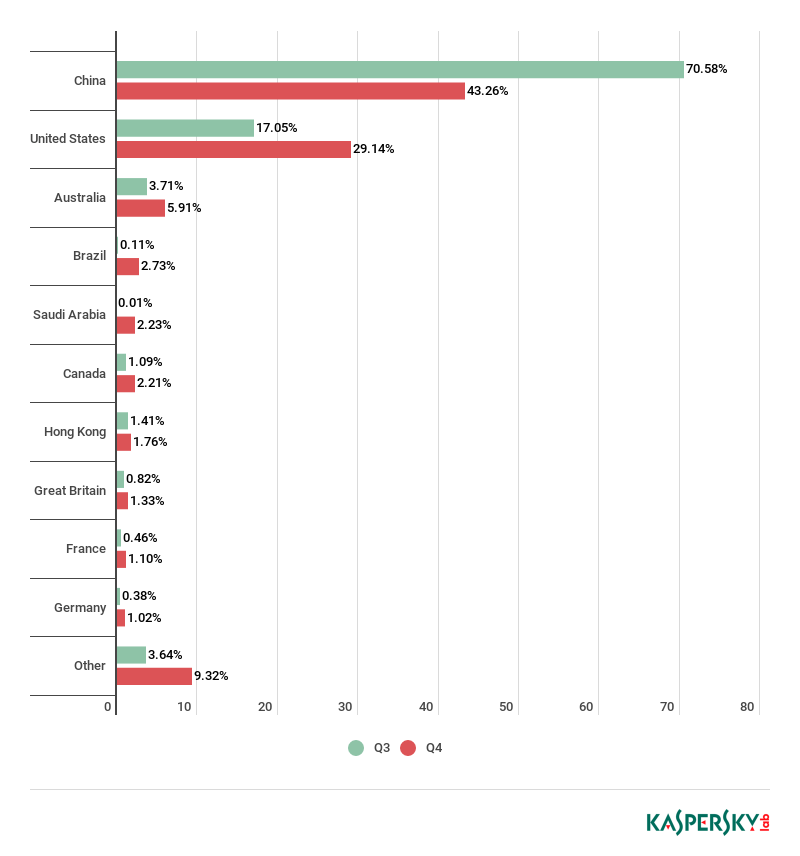
\includegraphics[scale=0.5]{figures/en-ddos-by-countries.png}
    \caption{在2018年Q3和Q4中,世界各国受DDoS攻击分布}
    \label{fig:ddos_countries}
\end{figure}

DoS攻击的危害性很大,而且它的实现形式也是各不相同。在所有的DoS攻击种类中,低速率服务拒绝(Low-rate Denial of Service, LDoS)攻击\cite{LDoS}是一种针对良性TCP流最有效的一种攻击。和直接发送大量流量的洪泛方式不同,它仅通过发送周期性的脉冲低速流就可以持续迫使TCP流进入超时重传(Retransmission TimeOut,RTO)的等待阶段,造成TCP流吞吐量显著下降的可怕后果。而且由于LDoS攻击的并非洪泛的方式,平均速率很低。相对于洪泛方式的DoS攻击,LDoS攻击更加难以被检测,而且,LDoS攻击以分布式方式实现的时候,LDoS攻击的隐蔽性更加强。
% Among all kinds of DoS attacks, the low-rate TCP attack~\cite{b20} is essentially the most efficient in terms of causing damage to benign TCP flows. Instead of directly sending a huge amount of traffic, it generates periodically pulsing low-rate flows to cause continuous retransmission of benign TCP flows, which results in significant throughput degradation. Due to the low rate, such attack is more difficult to be detected compared to flooding-based attacks. Moreover, the attack can be launched in a distributed mode, which further increases its stealthiness.

LDoS攻击对基于TCP协议发展起来的应用有非常大的影响,包括很多应用层的协议,例如BGP协议和HTTP协议。

有的研究\cite{b2}讨论了LDoS对BGP协议的影响。在使用LDoS攻击对运行BGP协议的网络进行干扰的情况下,BGP的控制平面误认为某条链路故障,导致该网络重新计算路径。因此,利用LDoS攻击可以迫使运行BGP协议的网络重复计算路径,不但可以消耗控制平面的计算资源,甚至还会引发BGP的路由震荡。

有的研究\cite{Maci2007LoRDAS}针对HTTP协议提出了LDoS攻击的变种攻击LoRDAS。该类攻击能够以极小的代价就能持续占用HTTP的服务器队列资源,从而使正常的HTTP请求无法得到服务器的响应,给基于HTTP协议的网络造成极大的影响。


因此,由LDoS攻击引起的安全问题也受到了重视。目前,为了有效的防御LDoS攻击,很多相应的对抗方案已经被提出来。大部分的解决方案\cite{b1,b4, b6, b7, b22}通过使用数字信号处理(Digital Signal Processing, DSP)技术来提取频域特征。只有采集数据流的周期合适的情况下,方案才能提取频域特征。然而,现行的方案都是采用一个固定的采样周期,来检测攻击流,这样会导致一些具有短周期的LDoS攻击流无法被检测出来。除此之外,这些方案都没有考虑限制被识别的攻击流的方法。有一些方案采用被动的防御方案来缓解LDoS攻击,不过,这些方案都没有识别攻击流,这些方案包括在主机上对TCP协议栈的RTO值进行随机化\cite{b17}和修改交换机上丢包机制的公平性规则\cite{b8}。因为这样的修改涉及到用户的网络协议栈或者交换机上面的硬件,所以这样的被动防御方案很难部署在大量的交换机上面。
%To effectively defend against the attack, several countermeasures have been proposed. Most defense solutions~\cite{b1,b4, b6, b7, b22} identify the attack flows by applying digital signal processing (DSP) techniques to extract frequency-domain characteristics. Such characteristics can only be well depicted when a proper sampling period of collecting flow statistics is set. However, existing methods apply a fixed sampling period, which may fail to detect attack flows with short periods. Besides, they do not consider how to throttle the identified flows. A few countermeasures adapt passive methods to mitigate the low-rate TCP attack without identifying attack flows, such as randomizing RTO of the TCP protocol stack in hosts\cite{b17} and modifying the fairness mechanism of dropping packets in the switches \cite{b8}. The passive defense solutions are not easy to be deployed in practice due to the modification of the network protocol stack in hosts or hardware in switches.

近来,软件定义网络(Software-Defined Networking, SDN)作为一个很有潜力的新型网络出现,改变了现行的网络架构的限制。首先,SDN网络将网络的控制平面从下层的路由器和交换机中分离出来,这样下层的交换机只需要负责数据平面,即转发数据流。其次,通过将数据平面和控制平面分离,SDN将控制逻辑放在中心控制器上,而交换机则负责数据的转发,这能够较为简单的配置网络和执行新的网络策略。而且,由于交换机只要与控制器完成连接,就可以接入已有网络并且不需要重复配置就能够执行统一的策略。



\begin{figure}
    \centering
    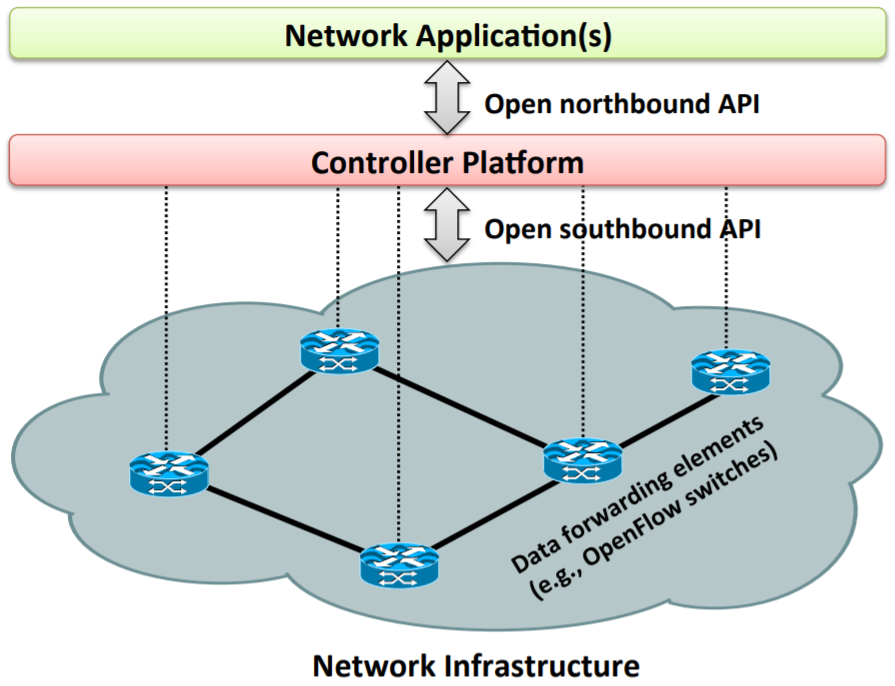
\includegraphics[scale=0.5]{figures/SDNnetwork.png}
    \caption{SDN网络架构}
    \label{fig:sdnfig}
\end{figure}

由于SDN是中心控制网络,控制平面和转发平面分离,通过编程灵活地制定网络安全策略能够达到比传统网络更加好的效果,所以,它在对抗DoS攻击上面有很多的优势。传统的网络设备上可以帮助识别DoS攻击的路由表项的匹配字段的数量优先,而且对于每个交换机而言,该设备仅仅自身的转发信息,若是在某个端口处的确认了DoS攻击,需要上游的设备配合定位攻击源。更有甚者,采用分布式的方式,很可能在定位攻击源的时候丢失攻击源的信息。

因此,很多基于SDN实现的方案~\cite{b9, b16, b11, b23, b24}被提出来防御各种各样的DoS攻击。但是,已有的方案都将注意力集中在防御洪泛式的DoS攻击。他们都没有考虑到如何检测和缓解LDoS攻击。值得注意的是,LDoS攻击的攻击流特点与洪泛式攻击的特点是有很大差别的。在SDN网络中,可以首先利用SDN独有的带宽限制机制对重要的链路对攻击流进行限制,接下来,利用SDN控制器对于全网的控制力来定位攻击源,直接对攻击源进行限制,从而达到防御LDoS攻击的效果。
%Recently, Software-Defined Networking (SDN) has emerged as a promising network paradigm. Due to the centralized control and flexible programmability, it shows great benefits on defeating DoS attacks. Several SDN-based approaches~\cite{b9, b16, b11, b23, b24} have been proposed to defend against various DoS attacks. However, existing defenses focus on defeating flooding-based DoS attacks. They fail to consider how to detect and mitigate the low-rate TCP attack. Now that the attack has great differences on the characteristics of the attack flows compared to the flooding attacks.


\section{主要研究内容}
\label{sec:work}
本文中的研究的主要内容是SDN网络的安全问题,针对DoS攻击的特殊攻击方式LDoS攻击的防御机制进行研究。在真实网络环境下,实现了两种基于SDN的LDoS攻击防御方案,基于带宽保障的方案和基于动态周期性检测的方案。两种方案在限制LDoS攻击上都有不错的表现。部署了防御方案的系统后,TCP流都不会因为LDoS攻击进入超时重传状态中。同时,两种方案引入的开销也很低。本文在真实的SDN网络交换机上完成实验,并且对系统进行了评估。

本文首先介绍LDoS攻击防御的研究现状,然后对现行的SDN中的DoS攻击防御的研究进展进行讨论。接下来,本文通过分析LDoS攻击的特点,平均速率很低、瞬时速率很高、具有周期性的特点设计相应的防御方案,提出了两个方案来抵御LDoS攻击。第一种方案是基于带宽保障的方案,该方案通过Meter规则限制非TCP流的速率,保留了重要链路的TCP流所需要的带宽,不会让TCP流完全丢包;第二种方案是限制攻击源的方案,提出了基于周期性检测的LDoS攻击检测算法和基于平均欧式距离(Mean Euclidean Distance, MED)的恶意流判定算法,再利用SDN的全局视野,可以很快的找到攻击源,并对攻击源进行限制。第一种方案保障了重要链路的正常运行,该方案可以在LDoS攻击的突发出现的时候,给TCP流保留部分带宽而让TCP流不会完全丢包而进入超时重传的长时间等待,直到LDoS攻击的突发结束的时候,TCP流重新恢复正常的传输,因此,LDoS攻击所造成的影响会小很多。第二种方案是使用两种算法精准的识别攻击流,然后利用SDN的全局视野,根据定位的攻击流直接安装相应的规则来限制攻击。若是LDoS攻击流的数据无法进入SDN网络,则LDoS攻击就无法对SDN网络造成任何影响,因此,使用第二种方案可以达到比已有的解决方案更加好的效果。


\section{研究意义}
\label{sec:contribution}
LDoS攻击防御的问题还是需要去研究的。因为,在之前的工作中,传统网络的LDoS攻击的防御方案都有着其固有的缺陷,有的方案定位并且限制LDoS攻击源。有的方案需要对交换机或者主机进行比较大的修改。而且当新的设备接入网络的时候需要重新配置,相对比较复杂。而已有的SDN的DoS防御方案没有针对于LDoS攻击的相关研究。相较于之前的LDoS防御方案,基于SDN的LDoS防御方案能够拥有更好的效果。总结一下,本文的四个主要贡献点:

\begin{itemize}
    \item 本文综合分析了LDoS攻击的攻击原理,再分析了SDN的优势,提出了SDN中防御系统,它能够有效地防御LDoS攻击而且不需要对交换机或者协议做任何修改。
    \item 本文提出了一种方案能够保证良性TCP流的基本传输,该方案能够使用Meter规则限制非TCP流的速率,保证了TCP流传输所需要带宽。所以,TCP流不会由于LDoS攻击而进入超时重传的等待时间。
    \item 本文提出了一种精准识别和限制LDoS攻击的方案。通过两个精准识别LDoS恶意攻击流的算法,能够准确地识别攻击源,并对提出两种规则对被识别出的攻击流进行限制。
    \item 本文在真实的网络中,通过部署于Floodlight控制器上的LDoS防御系统,实现了单攻击源和分布式的LDoS攻击,并验证了本文防御系统的有效性,并对两种方案进行了评估。
\end{itemize}

\section{各章内容安排}
\label{sec:arrange}
本文一共分为6章,各章节的主要内容如下:

第\ref{cha:intro}章的内容为引言,讲述了本文的研究背景,分析了已有方案对于LDoS防御的局限性,并提出了基于SDN的LDoS攻击防御方案,简要地分析说明了两种防御方案,并在最后总结了本文研究的意义。

第\ref{cha:relatedWork}章的内容为相关研究介绍,对目前LDoS攻击的相关防御工作的典型性方法进行分析,同时对SDN中DoS攻击的相关防御工作进行讨论。

第\ref{cha:LDoS}章主要介绍LDoS攻击的原理,分析LDoS攻击的特征,并且对LDoS的各种种类展开分析,最后对低速率分布式服务拒绝(Low-rate Distributed Denial of Service, LDDoS)攻击进行讨论。

第\ref{cha:design}章的主要内容为防御系统的设计,主要是设计两种LDoS攻击的防御方案,即带宽保障方案与LDoS攻击流限制方案。系统性分析两种方案的设计思想与对应的场景。

第\ref{cha:experiment}章的主要内容为实验总结和分析。在真实的SDN网络中,通过Floodlight分别部署两种方案的防御系统。在单攻击源和分布式LDoS攻击下,验证两种方案的的有效性。最后,对比两方案的特点,同时对两者方案进行全方位的比较和评估。

第\ref{cha:conclusion}章的主要内容为对本文的防御方案进行总结,并且对未来的工作进行探讨。
\chapter{相关研究综述}
\label{cha:relatedWork}

本章的主要内容包括两个部分,第一部分为介绍已有的LDoS攻击的防御方案,第二部分为介绍SDN中DoS攻击对策防御工作。

\section{LDoS的已有防御方案}
\label{chap2:LDoSwork}
之前已经有不少的LDoS攻击的防御方案被提出,经过实验,很多方案都能够对LDoS攻击进行有效的防御,其中。LDoS攻击的防御已有的防御方案主要有三种分类:基于时频域分析的类型、基于转发队列处理的类型和修改协议的类型。以下是对三种类型的方案的讨论。


\subsection{基于时频域分析的LDoS防御方案}
\label{chap2:TFanalysis}

Sun.H\cite{b4}等专家设计了基于动态时间规整(Dynamic Time Warping, DTW)算法的分布式检测方案。该方案提出了分布式LDoS攻击模型,在该模型下对LDoS的攻击流的数据进行规范化,将速率比较低的部分先进行过滤,这样可以对背景流量进行处理。然后,使用DTW算法来精准和有效地识别LDoS攻击,通过提取预定义的LDoS攻击模型特征与过滤后流量的特征对比来判定LDoS攻击流。接下来,提出了分布式系统来有效的区分攻击流和正常流,并对LDoS攻击流进行抑制。不过,依然存在一定的不足。在防御分布式LDoS的模型中,并不能对攻击源进行定位。

Chen.Y\cite{b7}等人提出了协同检测过滤(collaborative detection and filtering, CDF)方法来对LDoS攻击进行防御。该方案对所有的TCP/UDP流进行离散傅里叶变换(DFT)然后对他们的功率谱密度(Power Spectrum Density , PSD)进行分析,LDoS攻击流的功率谱密度的低频部分与正常流不一样,因为LDoS具有周期性,因此,LDoS攻击流在低频部分功率会相对更高。根据这个特征,该方案就能够对所有的流进行区分。不过,该方案需要的采样频率相对比较高,对计算资源的消耗相对比较高。

吴志军\cite{wuLDoSdetect}等学者提出了基于时间窗统计的LDoS防御方案。其核心思想是在网络流吞吐量下降的时候,利用时间窗去统计出现的突变脉冲数量,再根据数量多少去判断攻击是否出现。该类算法拥有比较好的识别率和误报率。但是,该方案只能检测出LDoS攻击流,却无法限制LDoS攻击,同时也存在着采样周期如何设定的问题。



\subsection{基于队列转发处理的LDoS防御方案}
\label{chap2:queanalysis}
Kwok.Y.K\cite{b22}提出了一种动态队列管理技术,该技术的核心思想就对数据流进行加权,然后对可疑流进行限制。该方案通过安装流表(flow table)来累计每个流的转发数据,如果通过流表在一段时间内观察到有段时间的高速率脉冲,则标定该流为攻击流,并优先丢弃该流的数据包。该策略可以在对LDoS攻击流有很强的限制作用,但是存在很大的不足,对于良性UDP流的误判率很高。

Chang.C.W\cite{b8}提出了修改队列公平性的方案,该方案中,每个路由器维持一个计数器并统计每个可能的受害者的丢包速率。


\subsection{修改协议的LDoS解决方案}
\label{chap2:promodify}

\section{SDN中DoS攻击的防御方案}
SDN作为一个新型网络,给DoS攻击的防御工作提供了新的思路,打破了之前的DoS攻击防御的限制,使用SDN的特性,采用新的方案更加有效的对LDoS攻击进行防御。其中包括两类比较典型的DoS防御方案,基于信息收发对称性的分析和动态变化带宽来检测DoS攻击。

\subsection{基于信息收发对称性的方案}
\label{chap2:srbalance}


\subsection{基于动态变化带宽的方案}
\label{chap2:dynamicbandwidth}

\chapter{LDoS攻击原理与形式介绍}
\label{cha:LDoS}

本章的主要内容是对LDoS攻击进行探讨。首先对LDoS攻击原理进行说明。接下来,对LDoS攻击模型进行分析与说明。最后,对LDoS攻击的各类攻击形式进行分析和探讨。

\section{LDoS攻击原理}
\label{chap3:LDoSstate}

\subsection{TCP拥塞控制机制和超时重传机制}

此部分的主要内容为分析传输控制协议(Transmission Control Protocol,TCP)的拥塞控制机制与超时重传机制。首先讨论了不同时期提出的TCP拥塞控制机制,然后对超时重传机制(Retransmission Time Out, RTO)进行分析,探讨超时重传机制对TCP流的影响。

TCP协议是保证数据可靠的协议。对于任何基于TCP协议的数据流,都需要TCP拥塞控制机制,因为该机制可以对网络进行有效的调节。在网络中,所有的流都想让自己的数据尽快的传输,但是,所有流尽可能传输的结果容易造成路由器或者链路的负载过大,引发网络拥塞,导致所有流都无法传输数据。因此,网络拥塞控制对于网络是必不可少的,而TCP拥塞控制是为了给TCP流提供合适的竞争方式。

在传输层中TCP协议实现了拥塞控制机制。TCP拥塞控制机制也并非一成不变的,针对不同的场景,TCP拥塞控制的策略也会不同,很多研究对TCP拥塞控制机制进行了探索。

最早的拥塞控制机制是1988年由Jacobson.V\cite{Jacobson1988Congestion}提出的TCP Reno版本,该方案的主要是由慢启动、拥塞避免、快重传和快恢复四个部分组成,大部分的拥塞控制方案都是以该方案作为基础进行提升的,由于该方案设计的时候有些方面未曾考虑,因此,该方案仅适用于低延迟、低带宽的网络。
在1994年由O’Malley.S.W\cite{O1994TCP}提出的TCP Vegas版本,该方案通过RTT来精准的预测带宽的变化,判断网络的可用带宽。不过,该方案适用于只存在这一种算法的时候。
在2008年,由Ha.S\cite{Ha2008CUBIC}提出的TCP Cubic方案,该方案使用立方函数作为拥塞窗口的增长函数,因此能够在不出现丢包的情况下,保持自己的传输速率。该方案能够尽可能的利用网络剩余带宽,适用于高带宽、丢包少的网络。
2017年由Cardwell.N\cite{Cardwell2017BBR}提出的TCP BBR版本,该算法在谷歌使用之后,极大的提升了数据传输性能。该算法认为当网络中的数据包总量高于网络中可存放数据包总量的时候会产生拥塞,就会限制窗口,因此,在带宽高、延迟高还有一定丢包率的情况下,降低时延并且保证带宽。
此外,2013年由Winstein.K\cite{Winstein2013Remy}提出的Remy算法采用机器学习的方式生成拥塞控制形式。因此,该算法适用于复杂的网络环境。

拥塞控制机制并非一成不变的,不同的方案有不同的适应场景,但是,这些方案都遵循着超时重传机制。在网络极其拥塞的情况下,TCP协议的发送端与接收端都收不到数据包,此时为了保证数据稳定的传输,TCP协议的发送端会进入指数退避阶段,将发送窗口改为1,避免网络进一步拥塞。在超时重传机制中,TCP流依靠RTO计时器来不定期探测网络拥塞状况。在TCP协议运行的过程中,RTO计时器中的值是由根据往返时间(Round-Trip Time,RTT)实时计算得到的。

TCP的发送端维持两个变量,平滑往返时间(Smoothed Round-Trip Time, SRTT)和往返时间变化量(Round-Trip Time VARiation, RTTVAR)。根据RFC2988\cite{2000Computing}的设定,RTO的实时计算结果与SRTT、RTTVAR两个变量相关。当TCP的发送端与接收端完成一次测量RTT之后,发送端将RTO计时器设置为3秒。
当第一次测量获得的RTT,记为$R'$,主机设置SRTT = $R'$,RTTVAR = $R' / 2$,RTO = SRTT + max(G, 4RTTVAR),此处的G被标记为时钟粒度(一般情况下,$\leq$100毫秒)。当获得一个RTT的值$R'$之后,RTTVAR和SRTT的计算公式如下:
%记为

\begin{center}
    RTTVAR = (1 - $\beta '$) RTTVAR + $\beta '$ |SRTT - $R'$|
\vspace{-0.1in}
\end{center}

\begin{center}
    SRTT = (1 - $\alpha '$) SRTT + $\alpha ' R'$
\end{center}

其中,有文献\cite{Jacobson1988Congestion}推荐设置$\alpha '$ = 1/8, $\beta '$ = 1/4。


通过对RTTVAR和SRTT进行更新之后,TCP发送端RTO的计算公式如下:
\begin{center}
    RTO = max(minRTO, SRTT + max(G,4 RTTVAR))
\end{center}

在Linux系统中,一般而言RTO计时器的最小值(minRTO)设置为0.2秒,因此,在推荐的参数中,延迟低的网络RTO基本是0.2秒。

接下来,对超时重传管理机制中RTO计时器进行控制的流程进行分析。若是在某一时刻$t_0$,一个序号为$n$的数据包有TCP的发送端发送,此时一个初始RTO值设为0.2秒的RTO计时器开始计时,如果$n$号的数据包丢失了或者说接收端重复发送的三个ACK包都没被发送包接收。当RTO计时器算到0.2秒的时候,则这个流就会被认为超时。此时,发送端进入指数退避阶段,发送端将拥塞控制的窗口置为1,并且让RTO计时器的值加倍,变为400毫秒,重传序号为$n$的未曾接收到ACK的数据包,并且重置RTO计时器为新的RTO的值。
%对超时重传管理机制通过(中)RTO计时器进行控制的流程进行分析
若是序号为$n$的数据包再次丢失,则发送端持续保持,发送端将保持在指数退避阶段,而RTO计时器将会等待400毫秒。也就是说在$t_0$ + 0.6s的时候,RTO的值将被设为800毫秒,并重复此过程。

若是序号为$n$的数据包的数据包成功的$t_0$ + 0.2s之前接收到该数据包,例如在$t$+ RTT的时刻接收到$n$号数据包,则TCP发送端退出指数退避阶段并将RTO的值置为0.2秒,又开始正常的传输。

\subsection{LDoS攻击原理}
此部分的主要内容对LDoS攻击原理进行分析,阐述如何利用TCP的超时重传机制对来实现DoS攻击。

上述的超时机制对于拥塞控制是十分重要的,因为在网络十分拥塞的情况下,发送少量的数据包先进行探测网络的可达性是必要的。但是,这样的超时重传机制也会给网络带来很大的风险,比如给特定的低速率攻击能够利用该机制对TCP流产生极大的影响。

若是一个攻击者针对TCP流,通过发送周期性的短时间高速突发来迫使该流重复进入超时重传状态。攻击的突发持续时间必须得超过RTT的时间,需要RTO为攻击的周期的整数倍数,例如,RTO,RTO/2,RTO/3等。受害者的吞吐量被限制待到近乎为0的程度。与此同时,由于该攻击的平均速率较低,不容易被DoS的对抗机制所检测。

\begin{figure}
    \centering
    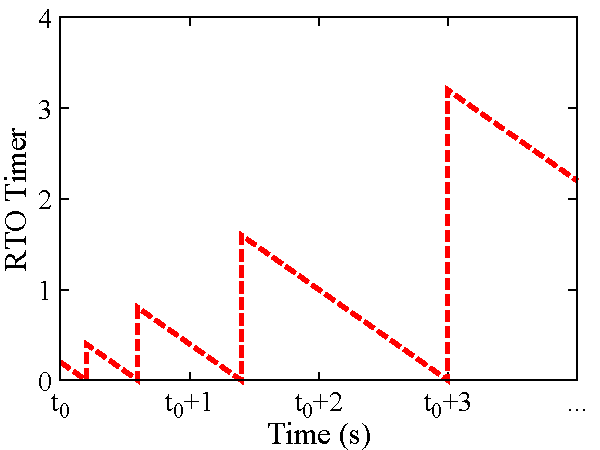
\includegraphics[scale=0.75]{RTO_timer}
    \caption{$t_0$时刻发动LDoS攻击之后,RTO计时器变化情况}
    \label{fig:rto-timer}
\end{figure}

首先考虑最简单的情况,若是一个攻击者仅仅针对一条TCP流进行攻击,攻击者在$t_0$时刻开始展开攻击,开始发送短时间的高速突发,就像图\ref{fig:rto-timer}展示的那样,根据RTO计时器的初始值为0.2秒,该TCP流会等待0.2秒。如果攻击者在$t_0$ + 0.2和$t_0$ + 0.2 + 2RTT的时间内进行短时间的突发流进行攻击,则TCP流将不得不等待额外的0.4秒。通过在$t$= $t_0$ + 0.6, $t_0$ + 1.4等点创造类似的攻击,就能够不断迫使该TCP流进入超时重传状态。因此,可以得到针对某一特定TCP流的DoS攻击流的形式,如图\ref{fig:rate-min-LDoS}所示。

\begin{figure}
    \centering
    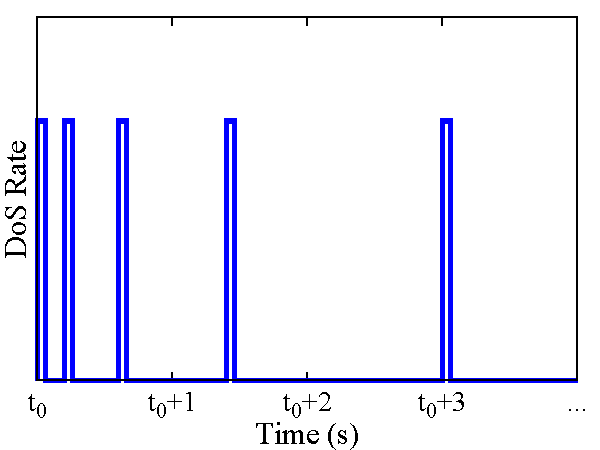
\includegraphics[scale=0.75]{rate-min-LDoS}
    \caption{高效的低速攻击方案}
    \label{fig:rate-min-LDoS}
\end{figure}

图\ref{fig:rate-min-LDoS}的攻击形式能够以最小的平均攻击速率使一个TCP流不断进入超时重传状态。但是,该形式却存在一个很大的弊端,若是在某一次攻击突发没有让ACK包被丢弃,则RTO计时器会重置为初始值,这样会使得该形式失效。因此,该形式虽然效率高,平均速率低,但是,并不适合于用作LDoS的基础形式。


\section{LDoS攻击模型}
\label{chap3:LDoS-model}
LDoS攻击形式需要一定的稳定性,不能因为偶尔出现的特殊情况就失去效果,考虑到这一点,使用周期性“方波”形式的UDP流作为LDoS攻击的基础形式能够获得比较好的效果。如图\ref{fig:LDoS}所示,其中攻击者可以通过发送周期为$T$,每次突发持续时间为$L$,突发速率为$R$的LDoS攻击流来对TCP流进行攻击。此时,可以用三个参数($T$,$L$,$R$)来描述LDoS攻击流。使用$\eta$来表示$\frac{L}{T}$的比值。

在这里,先以超时重传机制作为目标,分析LDoS攻击模型。LDoS攻击迫使TCP流进入超时重传状态是需要满足一定的条件的。首先,速率$R$必须足够大来引起丢包,也就是说,$R$与其他的流量混合起来一定要超过链路容量。其次,突发持续时间$L$必须足够长来引起丢包,但是也要足够短来避免检测。RTO计时器的初始值必须是周期$T$整数倍,为了使攻击的平均流量最小,本文将$T$设为minRTO,这样就能够满足LDoS攻击实现的条件。

\begin{figure}
    \centering
    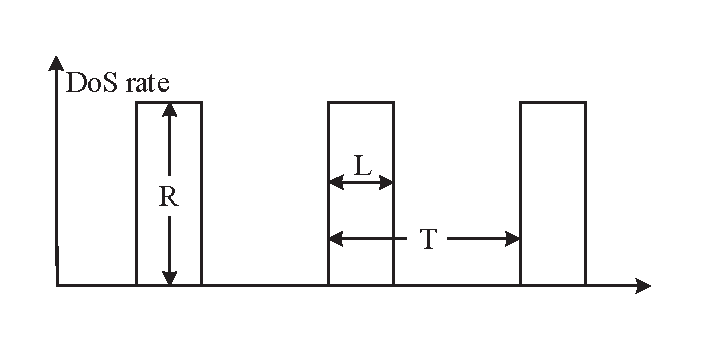
\includegraphics[scale=0.75]{LDoS}
    \caption{LDoS攻击形式}
    \label{fig:LDoS}
\end{figure}

前面讨论了针对一条攻击流的考虑LDoS攻击的情景,可以得到LDoS攻击模型,如图\ref{fig:model}所示,n条拥有不同RTT的TCP流和一条LDoS攻击流通过一个瓶颈队列。将RTT$_{i}$标记为第i条TCP流的RTT,其中i=1,…,$n$。LDoS攻击起效需要满足下面的条件:
\begin{itemize}
    \item 突发持续时间$L \geq RTT_i $
    \item minRTO > SRTT$_i$ + 4*RTTVAR$_i$
\end{itemize}

通过之前的分析可以得出一个结论,周期性的高速突发能够创造一段“停滞”状态,在这种状态下,丢包率很高,如果这种状态维持的时间超过RTT的时间规模,即$L \geq RTT_i$,则由LDoS的攻击突发引起的拥塞将维持足够长的时间来迫使所有的TCP流进入超时重传状态。除此之外,当且仅当minRTO > SRTT$_i$ + 4*RTTVAR$_i$的时候,则所有TCP流的RTO计时器的值就会统一为minRTO,这样攻击者就能够知道TCP流的RTO计时器的值。在这种情况下,能够排除影响LDoS攻击的两个重要的问题,第一个问题是不同的TCP流RTT不同;第二个问题是不同的TCP流RTO计时器的值不同。这样,LDoS攻击就能够对满足这两个条件的TCP流进行攻击。



% 接下来,考虑如果有TCP流不满足上述两个条件其中任何一个甚至两个都不满足,LDoS攻击的效果就会不一样。如果一些TCP流只有一部分满足上面两个条件,则他们的吞吐量将会降低至近乎为0的程度,而不满足上述条件的则吞吐量下降,下降的之后的标准化吞吐量由公式\ref{equ:thputsurvive}来描述。

% \begin{equation}
%     \label{equ:thputsurvive}
%     NT = \frac{\lceil \frac{minRTO}{T}\rceil T - minRTO}{T}.
% \end{equation}

\begin{figure}
    \centering
    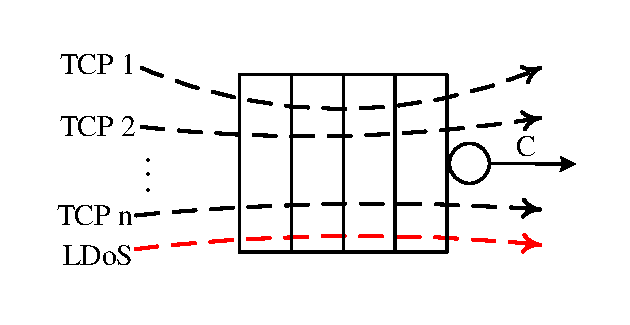
\includegraphics[scale=1]{queue}
    \caption{LDoS攻击模型}
    \label{fig:model}
\end{figure}

\section{各种类型的LDoS攻击}
\label{chap3:LDoStypes}
在LDoS攻击的基础形式被提出来之后,各种类型的LDoS攻击被提出来,根据目标的不同设定相应的参数能达到不同的攻击效果,例如基于超时重传机制的LDoS就能够迫使TCP流不断地进入超时重传机制,基于TCP的和式增加,积式减少(Additive Increase Multiplicative Decrease,AIMD)机制的LDoS能够迫使TCP流频繁地进入快恢复的状态。

根据Luo.X\cite{Luo2005OnAN}提出的方案,有两种LDoS攻击类型:第一种LDoS攻击可以继续利用超时重传机制降低TCP流的吞吐量;第二种LDoS攻击利用TCP的AIMD机制来降低TCP流的吞吐流量。第一种LDoS攻击同样需要图\ref{fig:LDoS}作为基础模型,$R$需要达到足够引起丢包,$L$需要长到引发ACK包丢失,$T$设定为比minRTO的值大一些。这样的LDoS攻击能够让TCP大部分的时间处于超时重传状态中,TCP流吞吐量依然降低了,但是并不能到近乎为0的程度。该方案的RTO计时器变化曲线如图\ref{fig:rto-timer-1}所示。由于该方案不需要与minRTO成倍数关系,所以比较好实现。第二种LDoS攻击是利用AIMD机制完成攻击。在通常的AIMD算法中,如果某一TCP流的滑动窗口大小为W,则由于一次短时间的高速突发引起该TCP流的数据包丢失,但是相应的ACK数据包到达了发送端,则TCP流不会进入超时重传状态,而TCP流的滑动窗口会下降至W/2。从此之后,该TCP流的滑动窗口大小每个RTT都增长1。针对TCP的AIMD机制的LDoS攻击同样被用来降低TCP流的吞吐量。攻击形式依然如图\ref{fig:LDoS}所示,相同的是$R$依然需要达到足够引起丢包,不同的是,$L$需要长到引发部分丢包即可,$T$可以设定为比较小的值这样,TCP流就会不断地减小滑动窗口大小。上述两种方式都能有效的降低TCP流的吞吐量。

\begin{figure}
    \centering
    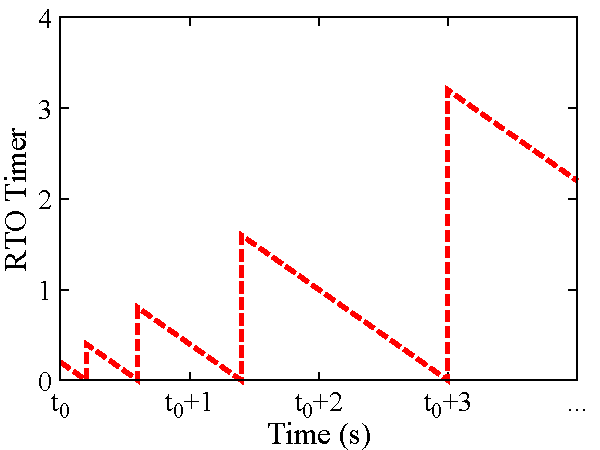
\includegraphics[scale=0.75]{RTO_timer}
    \caption{被新型利用超时重传机制的LDoS攻击的TCP流RTO计时器变化}
    \label{fig:rto-timer-1}
\end{figure}

也有研究\cite{b2}提出针对于BGP协议的LDoS攻击。由于BGP边界路由器之间使用TCP连接来交换可达性信息。在这样的情况下,使用对TCP流有很好效果的LDoS攻击将会对BGP会话的运行造成很大的影响。LDoS攻击对BGP会话的直接影响有两个:吞吐量下降和会话重置。第一个影响是吞吐量下降,因此BGP传递的信息会减少很多,BGP的更新速率将会非常缓慢,所以LDoS攻击大大降低了BGP的收敛速率。第二个影响就更加严重,BGP会话会重启,若是LDoS攻击流量持续时间足够长就能够引发BGP会话计时器超时,重启会话。BGP会话重启也将会加大的影响BGP的控制平面。

有文献\cite{Maci2007Evaluation}提出针对服务器队列的LDoS攻击。针对服务器的LDoS攻击首先对服务器进行洪泛攻击,让恶意请求使服务器的队列一处,然后,使用LDoS攻击形式去对服务器进行攻击,周期性的发送恶意请求给服务器,在每次预测到服务器的队列没有完全被使用的时候,就在那段时间里不断发送请求给服务器,直到服务器队列再次溢出。攻击的周期为一个服务器接受请求到下发回复的时间长度。该类LDoS攻击通过消耗服务器的队列资源使服务器拒绝服务,而且由于发送请求的速率相对比较低且均为合法流量,因此,难以被检测。

还存在有针对应用层HTTP协议的的LDoS攻击\footnote{https://blogs.akamai.com/2013/09/slow-dos-on-the-rise.html}。该类攻击有三种类型:Slow HTTP Headers,Slow HTTP Post和Slow Read Attack。这三种类型攻击都是通过发送大量合法的请求给服务器来创造大量的服务器连接,并发送周期性的合法请求来长期维持这些连接,在大量占用了服务器链接资源池的资源之后,一直不释放,则链接资源池被沾满,造成服务器的服务拒绝攻击。而且由于合法请求造成的资源被占用,难以被释放。
%占用-释放
\section{低速率分布式服务拒绝攻击}


前文所分析的LDoS攻击都是有某一主机作为攻击者集中实现的,这样便于部署攻击并保证攻击形式能够按照要求实现。低速率分布式服务拒绝(Low-rate Distributed Denial of Service, LDDoS)攻击作为LDoS的分布式部署方式,相较于单攻击源的LDoS攻击拥有很多的优势。首先,若是想对性能比较好的交换机上使用LDoS攻击,单主机的性能可能达不到要求,需要多主机联合攻击。其次,作为分布式LDoS的每个攻击主机拥有更加低的平均速率,更加不易被检测出来。

部署分布式LDoS攻击是需要前提条件的,只有满足了一定条件才能实现分布式攻击。假设多个攻击主机想联合对某条TCP流$f$进行攻击,则需要这些攻击主机在该TCP流经过的一个交换机$s_r$上的链路$l$进行攻击,且攻击主机的流量需要以一定的规则汇聚到$l$上。所以,攻击主机需要满足两个条件:(1)每个攻击主机都有一条攻击路径经过$l$;(2)所有主机需要计算好时间,使得流量到$l$处时刚好形成LDoS攻击。除此之外,攻击主机还需要发送足够的突发流量来拥塞这个瓶颈链路$l$,并设置好攻击周期来避免检测。

在满足了上述两个条件之后,同步的分布式LDoS攻击就具备了拥塞TCP流的能力。在多个攻击主机上运行的LDoS攻击与单一攻击源的单独流量更低,也存在很多不同的形式,接下来,以两个主机联合攻击来展示迫使TCP流持续保持超时重传状态的分布式LDoS攻击。


\begin{figure}
    \vspace{-0.2in}
    \begin{subfigure}{1\textwidth}
        \centering
        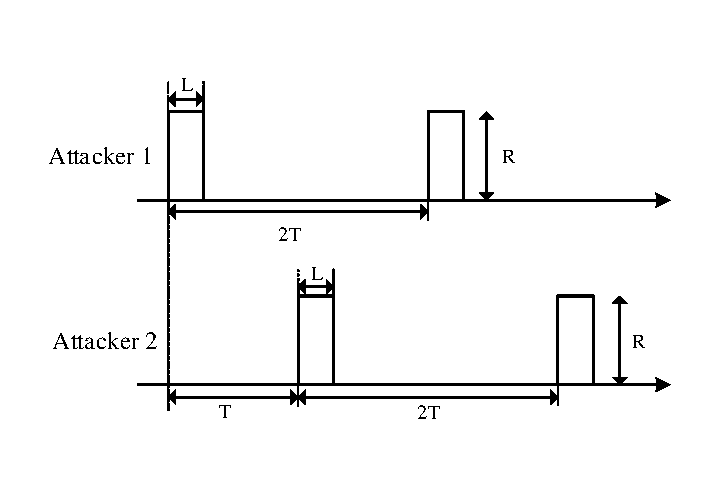
\includegraphics[scale=0.75]{lddos2}
        \caption{方案一}
        \label{fig:lldos1}
    \end{subfigure}

    \begin{subfigure}{1\textwidth}
        \centering
        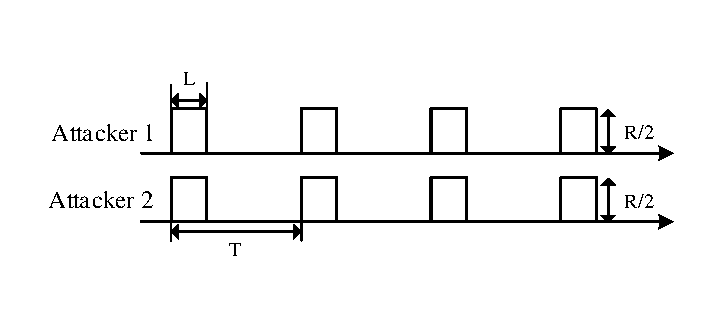
\includegraphics[scale=0.75]{lddos3}
        \caption{方案二}
        \label{fig:lldos2}
    \end{subfigure}

    \begin{subfigure}{1\textwidth}
        \centering
        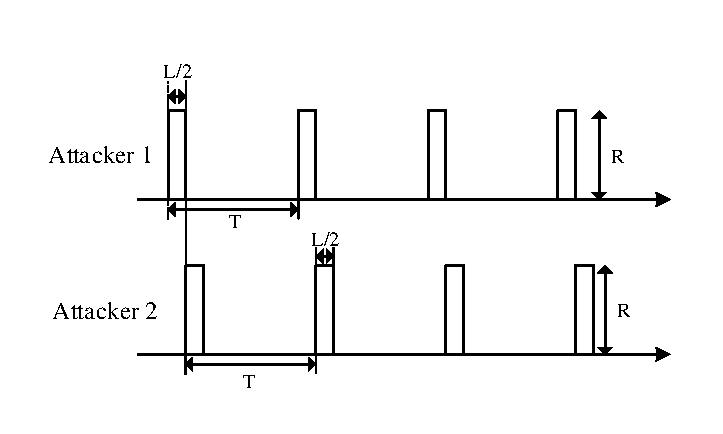
\includegraphics[scale=0.75]{lddos1}
        \caption{方案三}
        \label{fig:lldos3}
    \end{subfigure}


    \caption{分布式LDoS攻击}
    \label{ffig:lldos}
\end{figure}


% \begin{figure}
%     \centering
%     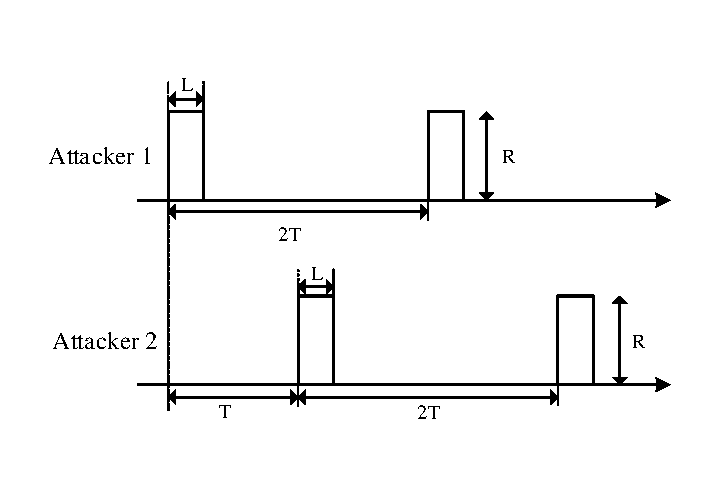
\includegraphics[scale=0.75]{lddos2}
%     \caption{分布式LDoS攻击的第一种方案}
%     \label{fig:lldos1}
% \end{figure}
图\ref{fig:lldos1}为分布式方案一,将该方案的两个流聚合,就可以得到一个参数为($R$,$L$,$T$)的LDoS。首先对第一种方案进行分析,假设攻击者1在零时刻发动了突发速率为$R$,周期为$2T$,每次突发持续时间为$L$的LDoS攻击,则TCP流$f$由于攻击进入超时重传状态。每次$t$ = 2i * T(i=0,1,2…)时刻的$f$可能出现的ACK数据包由于攻击者1的攻击流的拥塞而丢弃。攻击者2需要在$T$时刻发动突发速率为$R$,周期为$2T$,每次突发持续时间为$L$的LDoS攻击,则每次$t$ = (2i + 1) * T(i=0,1,2…)时刻的$f$可能出现的ACK数据包由于攻击者2的攻击流的拥塞而丢弃。至此,由于两个攻击者的拥塞,TCP流$f$的所有可能接受的的ACK报都丢失了,因此,该TCP流持续保持超时重传状态。

% \begin{figure}
%     \centering
%     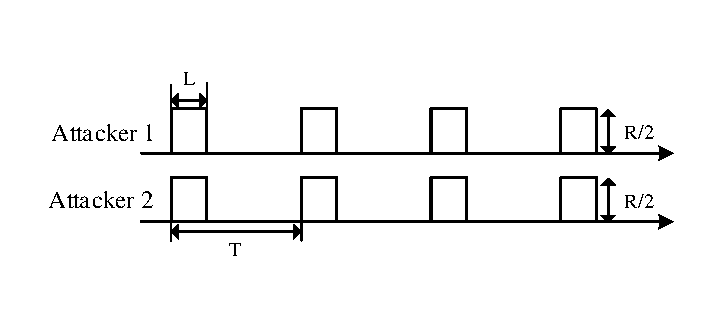
\includegraphics[scale=0.75]{lddos3}
%     \caption{分布式LDoS攻击的第二种方案}
%     \label{fig:lldos2}
% \end{figure}

图\ref{fig:lldos2}为分布式方案二。攻击者1在零时刻发动突发速率为$R/2$,周期为$T$,每次突发持续时间为$L$的LDoS攻击,若是只有攻击者1,则由于攻击突发速率不足,不能使队列拥塞并造成TCP流的丢包,所以,需要攻击者2与攻击者1在零时刻同步发动突发速率为$R/2$,周期为$T$,每次突发持续时间为$L$的LDoS攻击,攻击突发速率足够,因此,交换机的队列拥塞造成TCP流的包完全丢失,最终持续进入超时重传状态。

% \begin{figure}
%     \centering
%     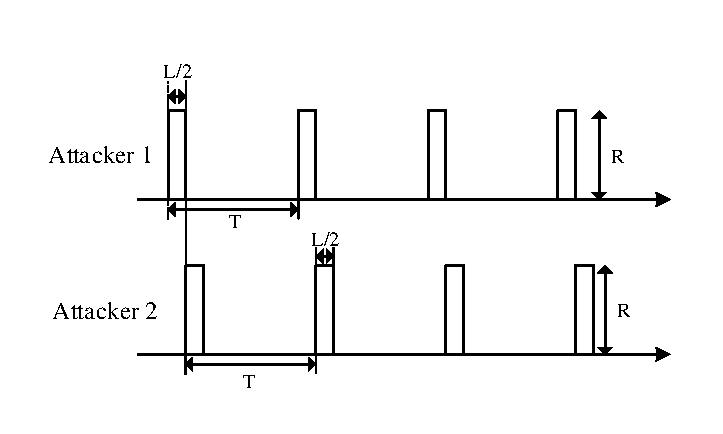
\includegraphics[scale=1=0.75]{lddos1}
%     \caption{分布式LDoS攻击的第三种方案}
%     \label{fig:lldos3}
% \end{figure}

图\ref{fig:lldos3}为分布式方案三。攻击者1在零时刻发动突发速率为$R$,周期为$T$,每次突发持续时间为$L/2$的LDoS攻击。若只有攻击者1的攻击,则由于突发持续时间不足,导致TCP流的ACK包可以为TCP发送端接收到,无法迫使TCP流进入超时重传状态。因此,需要攻击者2在$L/2$时刻,也发动突发速率为$R$,周期为$T$,每次突发持续时间为$L/2$的LDoS攻击。由于攻击者2的攻击在攻击者1结束的时候刚好出现,因此,延续了攻击者1的LDoS攻击的效果,TCP流的ACK包由于攻击者2的拥塞而丢失,所以该TCP流被迫进入超时重传机制。

以上三种方案分别在突发持续时间、突发峰值速率、突发周期上进行了分布式探索,三种方案都能够迫使TCP流保持超时重传状态,而且每个攻击主机都平均攻击速率相较于单一主机都有所下降,这样更易于逃避DoS防御机制的检测。


\chapter{SDN中LDoS防御方案设计}
\label{cha:design}
本章的主要内容为LDoS防御方案的设计。首先,对LDoS的特征进行分析,找到防御LDoS的关键点。然后,根据防御LDoS的要点,结合SDN的优势设计了SDN中防御LDoS的两种方案。最后,对两种方案的设计思想和实现方案进行探索和分析。本文是基于SDN中最经典的OpenFlow协议完成设计的。

\section{SDN中LDoS防御的关键点分析}
\label{chap4:keyanalysis}
前文已经对LDoS攻击的攻击形式进行了说明,本文首先分析单攻击源的LDoS攻击实现的关键点并找到合适的防御机制。LDoS攻击的核心思想就是通过周期性的引发TCP流丢包,触发TCP拥塞控制机制或者超时重传机制降低TCP流的吞吐量,最后达到以极低的流量使TCP流异常的目标。因此,本文防御LDoS有两种核心思想,第一种是采取措施使TCP流不丢包,第二种是找到并限制攻击源。

第一种思想是采取措施使得TCP流不丢包。通过前文可知,TCP流的丢包是由于LDoS的速率太高拥塞队列导致的。所以,只要交换机保护TCP流的最低通信需求,则TCP不会因为收不到任何包而进入超时重传状态。在SDN网络中,带宽保障可以通过SDN中特有的meter规则去实现,使用meter规则限制其他流的最高速率从而给TCP流提供有最低速率保障,则LDoS无法通过拥塞队列强迫TCP流完全丢包。从而达到防御LDoS攻击的效果。但是,这样的做法在LDoS攻击的突发到达的时候,速率依然会降得很低,而拥塞窗口也会相应的减小,因此,这种思想只能减轻攻击所造成的危害,但是不能完全消除LDoS攻击对TCP流的影响。

第二种思想是找到并且限制攻击源。在SDN网络中,所有的数据转发都是由流表规则匹配完成的,因此,在SDN中可以实现流级别的数据分析。由于LDoS攻击拥塞了某个交换机的队列才能实现攻击,因此,可以在交换机的端口处检测LDoS是否存在。LDoS攻击作为一个周期性的“方波”是能够由周期性来确认的,因此,在端口处只要能够确认有周期性的吞吐量变化,就能够确认攻击,再之后通过流级别的分析判断攻击流,最后,再对判断出来的攻击流的攻击源进行限制。使用这种思想来防御LDoS攻击就能够完全消除LDoS攻击流对TCP流的影响,但是,在攻击开始的时候TCP流会受到一定的影响,可能会出现部分TCP流进入超时重传状态,影响吞吐量。

\section{SDN中基于带宽保障的LDoS防御方案}
\label{chap4:bandguatee}

为了保证TCP流不进入超时重传状态,防御方案必须保证TCP流无论在什么情况下都不能丢包,结合SDN的特性,该方案结合OpenFlow的Meter规则来实现,可以最大程度利用SDN网络可以自由制定网络规则的特性。

首先,分析Meter规则是如何在SDN中运行的,才能制定相应的Meter规则防御LDoS攻击。Meter规则允许SDN实现各种各样的服务质量(Quality of Service,QoS)配置,其中就包括了速率限制。Meter规则能够直接与SDN中的流表规则绑定,这样Meter规则可以测量和控制所有与之绑定的流表规则的聚合速率,因此,Meter规则可以用来限制除TCP流以外的所有流聚合的速率。

\begin{table}[htbp]
	\centering  % 显示位置为中间
	\caption{Meter规则}  % 表格标题
	\label{table:meter}  % 用于索引表格的标签
	%字母的个数对应列数,|代表分割线
	% l代表左对齐,c代表居中,r代表右对齐
	\begin{tabular}{|c|c|c|}  
		\hline  % 表格的横线
        Meter Identifier & Meter Bands& Counters \\  % 表格中的内容,用&分开,\\表示下一行
        \hline
		
	\end{tabular}
\end{table}
%英文斜体字?
表\ref{table:meter}为SDN的Meter规则的主要内容。Meter Identifier是一个32比特的无符号整数,它能够用于唯一标识一个Meter规则。counters是统计与meter绑定的流表规则的统计相关数据,随时更新。其中,最重要的是Meter Bands,它是Meter规则控制和限制绑定聚合流的速率和处理包方式的部分。需要注意的是,每个Meter规则可以匹配多个Meter Band。表\ref{table:meterbands}为一个Meter Band部分,它由五个部分组成,首先是Band Type部分,这直接定义了速率超过限定速率以后,后面的包是如何处理的。此处有两种选项:一种为\emph{drop},这样它该Meter规则就可以被用来限制速率;另一种为\emph{dscp remark},这样就能增加数据包IP头中DSCP字段的丢弃优先级,可用于定义不同级别的服务。第二个参数是Meter规则限制的速率,它定义Meter规则最低适用的速率,若是速率高于该参数的数据包则需要根据Meter规则进行处理。Counters表示被该Meter Band处理的包的统计数据。Burst参数是本文需要调的一个重要参数,该参数定义了Meter Band的粒度。Type specific arguments表示band types有特殊的参数。

\begin{table}[htbp]
	\centering  % 显示位置为中间
	\caption{Meter Band}  % 表格标题
	\label{table:meterbands}  % 用于索引表格的标签
	%字母的个数对应列数,|代表分割线
	% l代表左对齐,c代表居中,r代表右对齐
	\begin{tabular}{|c|c|c|c|c|}  
		\hline  % 表格的横线
        Band Type & Rate & Burst & Counters & Type specific arguments \\  % 表格中的内容,用&分开,\\表示下一行
        \hline
		
	\end{tabular}
\end{table}

此方案使用Meter规则来实现对非TCP流的速率限制,这样就能够对LDoS攻击进行限制。但是,由于LDoS攻击具有一定的特殊性,普通配置Meter规则无法限制LDoS攻击,需要特殊的配置。首先,由于LDoS攻击会拥塞某个端口的队列,所以,对于每个激活的端口,都应当配置一个相应的Meter规则进行限制,对于从端口处发送非TCP数据的流表规则需要与该端口的Meter规则进行绑定,受该Meter规则的束缚。接下来,Meter规则的粒度也需要特殊的配置,默认的状态下,Meter规则是以1秒作为统计单位进行速率限制的,由于LDoS攻击的平均速率并不能满足Meter规则限制的需求,因此Meter Band设置的Burst参数需要重新配置。接下来,需要设置Rate参数的大小来限制非TCP聚合流的速率,设置的参数数值大了会影响其他正常流的速率,设置的值过小会使TCP流的窗口降至极小的程度,达不到限制LDoS攻击的效果。因此,研究该参数对吞吐量大小的影响非常重要。


基于带宽保障的LDoS防御方案可以分为两个模块完成。流程图如\ref{fig:meter-solution}所示。防御方案的第一模块为预配置Meter规则模块,控制器首先会检测所有激活端口,并给每个端口分配一个Meter规则,Meter规则需要调节Burst参数使得粒度在RTT级别大小,这样才能够有效的限制LDoS攻击的速率。其次,设置合理的Rate参数保证TCP流不进入超时重传机制的同时使滑动窗口不至于变得太小。设置Band Type为drop,这样就可以丢弃所有超速的包,保障了TCP流有一定的带宽可以使用。防御方案的第二个模块为流处理模块,有一个流进入交换机,则需要对该流进行区分处理。若是该流为TCP流,则该TCP流的流表不需要绑定任何Meter规则,这样它就不会被Meter规则所束缚,可以按照TCP拥塞控制的机制进行速率的控制。若是该流不是TCP流,则需要绑定Meter规则以保证该流不会对TCP流造成损害,特别是当该流为LDoS攻击流的时候,由于速率被控制,队列不会被该流所拥塞而造成TCP流丢包,TCP流就不会进入超时重传状态。


%图 窗口与burst size的关系图,窗口与限制速率关系	有无防御机制吞吐量对比图

\begin{figure}
    \centering
    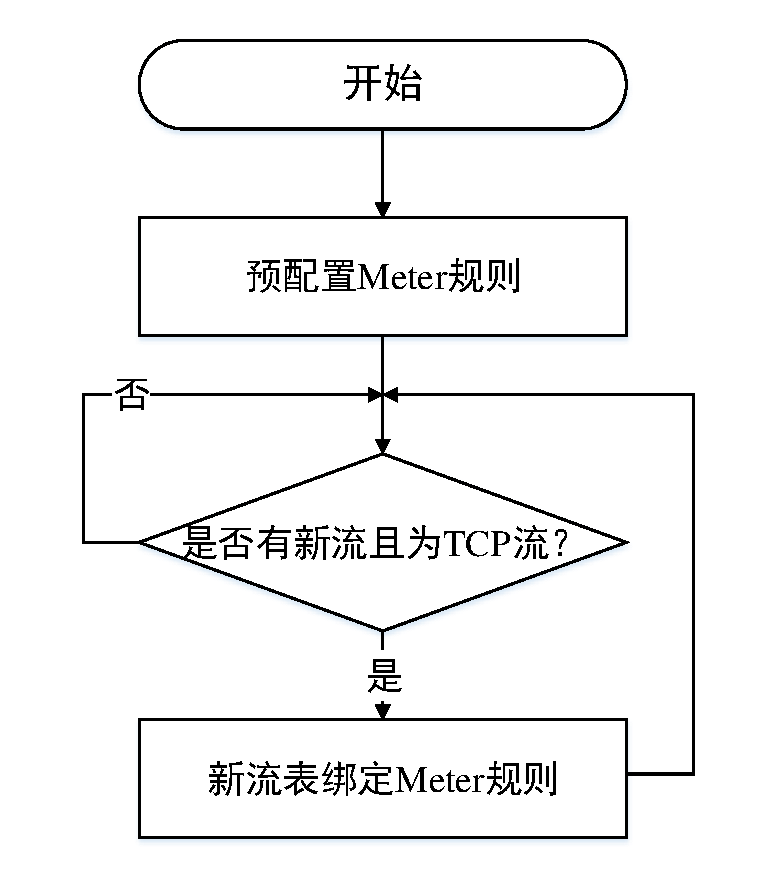
\includegraphics[scale=0.5]{meter-solution}
    \caption{基于带宽保障的LDoS防御方案流程图}
    \label{fig:meter-solution}
\end{figure}


\section{SDN中基于动态周期性检测的LDoS防御方案}
\label{chap4:SoftGuard}
已有SDN防御方案无法对LDoS限制的时候,为了保证SDN网络的正常传输,本文提出了基于动态周期性检测的方案。作为一个基于SDN的轻量级防御方案,该方案能够准确地识别并且有效地限制LDoS攻击。该方案分为三个模块,异常检测模块、攻击定位模块和攻击限制模块。每个模块都有特定的攻击,只有在一定的条件下激活才能发挥作用。因此,也最大程度的减轻了系统的负担。该方案是基于SDN中流表规则实现的,通过流表规则,SDN控制器能够获取交换机中各种有用的信息。

\subsection{SDN中相关流表规则分析}
\label{chap4:flowruleanalysis}

流表规则是SDN交换机中很重要的部分,所有的经过交换机的数据包都需要经过流表规则进行处理,这些数据包会优先寻找优先级比较高的流表规则进行匹配,这些流表规则可能有很多指令规则,其中比较重要的有两种,一种是将包从端口转发出交换机,另一种是转给交换机内的其他流表规则处理。表\ref{table:flowrule}为流表规则的主要内容。根据需求合理的配置流表规则的参数,能够实现对LDoS攻击的检测与限制。

本文对流表规则中重要的部分进行分析,制定合适的特制流表来防御LDoS攻击。在流表规则中,最重要的三个部分是匹配域(Match Fields)、优先级(Priority)和指令(Instructions)。匹配域一般是由入端口和数据包头部组成,也有其他可选项区域。优先级(Priority)是用来区分数据包优先匹配的规则的,若是同一个数据包同时匹配两个流表规则的匹配域,则该数据包会优先按照优先级高的流表规则的指令操作。通过匹配域和优先级可以使数据包确定匹配的流表规则,若是没有匹配上流表规则,就会将该数据包的包头上传控制器,请求相应的流表规则。在确认了流表规则之后,该数据包会按照流表规则的指令完成操作。流表规则还具备数据统计的功能,其中的计数器(Counters)就记录了很多重要的信息,其中包括了转发的数据包的数量和字节数,每当匹配到数据包时,计数器中的数据就会实时更新。流表规则中的Timeouts参数包括两个timeout参数,idle\_timeout和hard\_timeout。idle\_timeout若是一个非0的数值,则流表规则将在匹配最后一个包之后的idle\_timeout给定的时间后移除;idle\_timeout为0,则该参数不影响流表规则。hard\_timeout若是为非0的数值,则流表规则不管有没有匹配数据包,都会在hard\_timeout给定的时间后移除;hard\_timeout为0,则该参数不影响流表规则。若是idle\_timeout和hard\_timeout都为0,则流表规则永远存在,而且除了特定的指令外不会被删除。Cookie部分是控制器用于标识流表的不透明数据,该数据可以用来获取特定流表规则的信息,在处理数据包的时候不适用。Flags字段可用于出发特殊的消息给控制器。


\begin{table}[htbp]
	\centering  % 显示位置为中间13
	\caption{流表规则}  % 表格标题
	\label{table:flowrule}  % 用于索引表格的标签
	%字母的个数对应列数,|代表分割线
	% l代表左对齐,c代表居中,r代表右对齐
	\begin{tabular}{|c|c|c|c|c|c|c|}  
		\hline  % 表格的横线
        Match Fields & Priority & Counters & Instructions & Timeouts & Cookie & Flags \\  % 表格中的内容,用&分开,\\表示下一行
        \hline
		
	\end{tabular}
\end{table}

控制器通过以恒定的速率进行周期性的查询,可以获得每个流表规则中计数器的速率。对于不同应用,通过选择合适采样的周期可以尽可能减少控制器的带宽负载,同时也可以尽可能提高服务的质量。本文将每次查询的间隔时间长度标记为$T_s$,将以此采样间隔内的平均速率当做采样时刻的速率,用于不同的服务。公式\ref{eqa:rate}展示了从流表规则的数据中获取流表规则速率的方式。

\begin{equation}
	\label{eqa:rate}
	S(t) = \frac{Counter\_bytes(t) - Counter\_bytes(t - T_s)}{T_s}
\end{equation}

\subsection{总体设计}
\label{chap4:overview}

基于动态周期性检测的LDoS防御方案有三个模块,异常检测模块、攻击定位模块和攻击限制模块。整体框架如图\ref{fig:architecture}所示。其中异常检测模块是在交换机中给每个端口都安装了特制的流表规则用于统计检测TCP的聚合流量。由于异常检测模块并没有对所有流表规则进行检测,这样就减少了对于控制器的带宽开销。当异常检测模块检测到某个端口TCP流的聚合吞吐量下降的时候,就会激发攻击定位模块在这个异常端口处确认LDoS攻击、识别LDoS攻击流、并定位攻击源。确认LDoS攻击的关键点就是查看端口的聚合吞吐量是否存在周期性,由于LDoS攻击是由周期性的脉冲流组成的。攻击定位模块设计了适应性周期检测方法方法来预测LDoS攻击的周期。除此之外,攻击定位模块还用了平均欧氏距离(Mean Euclidean Distance,MED)从所有经过异常端口的流中识别出LDoS攻击流,然后通过SDN的全局视野找到攻击流的源端。最后,攻击限制模块将在LDoS攻击源的入口交换机处安装相应的限制规则以限制LDoS攻击流。

\begin{figure}
    \centering
    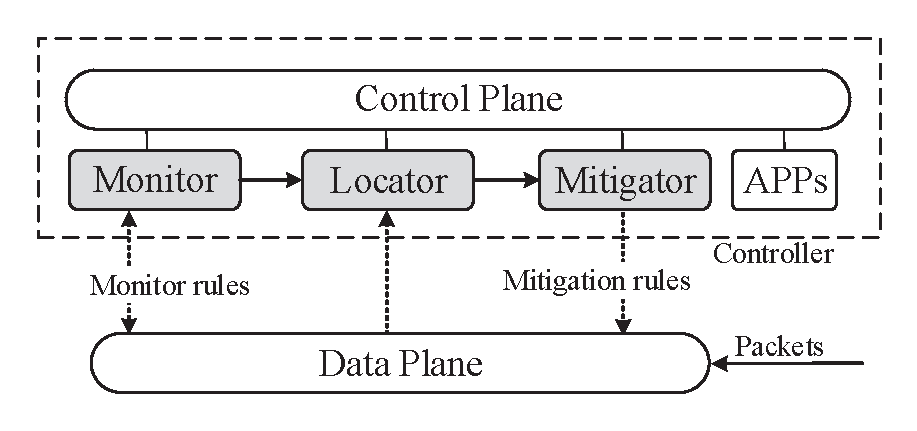
\includegraphics[scale=0.75]{architecture}
    \caption{基于带宽保障的LDoS防御方案流程图}
    \label{fig:architecture}
\end{figure}

\subsection{异常检测模块}
\label{chap4:Monitor}
异常检测模块的作用是在交换机上的每个端口处检测可能存在的LDoS攻击,并且激活其他模块来确认LDoS攻击。异常检测模块通过在每个交换机上安装检测流表规则在端口上来检测LDoS攻击。这些流表规则能够统计每个端口的TCP流的聚合吞吐量。异常检测模块通过周期性地获取这些流表规则的计数器数据就可以获知TCP流的聚合吞吐量变化情况。

异常检测模块首先从所有的数据包中分离出TCP数据包。然后,TCP数据包通过与这些特制的流表规则匹配,统计数据。接下来,再将这些TCP数据包转发给其他正常的流表规则进行处理。这些特制流表的匹配规则的匹配域加入转出端口信息,同时将优先级置为最高,以保证这些流表规则优先匹配数据包以统计TCP流的信息。接下来,特制的流表规则的指令为转发给其他正常流表规则进行处理,保证了这些流表规则只会统计TCP流的信息而不会干扰数据的传输。同时,异常检测模块需要把这些特制流表规则的idle\_timeout和hard\_timeout都设置为0以保证特制流表规则不会被删除,可以持续做数据的统计。

在交换机上安装特制流表规则后,异常检测模块按照算法\ref{alg:detection}检测TCP流的聚合吞吐量状态,若是TCP流的聚合吞吐量持续下降,则表示TCP流的聚合吞吐量下降明显,然后判断LDoS攻击是否可能出现,异常检测模块将会激活攻击定位模块来进行更深入精确的检测。算法\ref{alg:detection}展示了检测TCP吞吐量异常的伪代码。输入由吞吐量下降判定阈值$\alpha$和检测所得的序列$S$组成。输出为检测所得的结果$s$。$c$记录吞吐量持续下降的时间。如果$c$超过一个阈值$M$,$s$将会被标记为吞吐量异常,以此表示可能存在的LDoS攻击。同时检测到吞吐量异常的端口将被标记为异常端口。考虑控制器的带宽负载和模块的效率,设置异常检测模块的采样周期$T_s$为0.5秒,每次检测的时间长度为5秒。

\floatname{algorithm}{算法}
\renewcommand{\algorithmicrequire}{\textbf{输入:}}
\renewcommand{\algorithmicensure}{\textbf{输出:}}
\begin{algorithm}
	\small
	\caption{TCP流的聚合吞吐量异常检测}
	\label{alg:detection}
	\begin{algorithmic}[1]%ÿÐÐÏÔʾÐкÅ
	\Require $\alpha, S$;
	\Ensure $s$
	\State $c \gets 0$;
	\State $s \gets $吞吐量正常;
	\For{$(i=2 \rightarrow {len(S)})$}
		\If {$S_{i} < {\alpha} * S_{i - 1}$}
			\State $c \gets c + 1$;
		\Else 
			\State $c \gets 0$;
		\EndIf
		\If {$c {\ge} M$}
			\State $s \gets$ 吞吐量异常;
		\EndIf
	\EndFor
	\State \Return $s$
		
	\end{algorithmic}
\end{algorithm}

\subsection{攻击定位模块}
\label{chap4:Locator}

在异常检测模块激活了攻击检测模块之后,攻击检测模块对异常检测模块检测出的异常端口进行分析,确认LDoS攻击并识别LDoS攻击流。供给定位模块分为四个步骤。第一步,攻击定位模块对异常端口的总吞吐量进行二值化。第二步,攻击定位模块通过这些二值化后的吞吐量推断出异常端口吞吐量是否存在周期性。如果异常端口吞吐量存在周期性,则供给定位模块将确认异常端口正在被LDoS攻击所影响,因此,本文将确认被LDoS攻击所影响的端口称为受影响端口。攻击定位模块使用算法\ref{alg:port_locate}来确认异常端口是否为受影响端口。第三步,使用序列相似性来识别攻击流,通过平均欧式距离方法来判断攻击流。最后一步,找到攻击流的入口交换机上的端口,并且通知攻击限制模块来限制攻击流。




\subsubsection{吞吐量序列二值化}
\label{chap4:binarization}
通过采样获得的吞吐量序列在进行周期性判断之前需要进行处理。端口统计的数据包除了潜在的LDoS攻击数据包,也可能会包含在其他良性的流量影响周期性的判断。这些良性流量括三类:
\begin{itemize}
	\item 不会受到LDoS攻击和网络拥塞影响的UDP流
	\item LDoS未影响到的TCP流
	\item 其他经过该端口的更底层的数据流
\end{itemize}
这些良性流量不具备周期性,而且速率相较于LDoS的突发速率$R$要小很多。为了减少这些良性流量的影响,同时也为了更加便于提取周期性,攻击定位模块需要对流量进行二值化。攻击定位模块使用了阈值法进行二值化,假设该序列的最大吞吐量的值为$S_m$,设定二值化阈值为$\beta$,则吞吐量序列值中高于$\beta S_m$的地方置为1,吞吐量序列值中低于$\beta S_m$的地方置为0,这样就可以得到二值化序列。

\subsubsection{流量周期性检测}
为了确认LDoS攻击,攻击定位模块需要检测异常端口聚合流量周期$T$。所以,攻击定位模块能够通过检测二值化序列的周期$T_b$来推断周期$T$。假设某异常端口有周期为$T$的LDoS攻击流,控制器通过对异常端口的数据以合适的采样间隔$T_s$进行采样并进行二值化,获得二值化序列。通过提取二值化序列的功率谱密度的振幅最大值对应频率,就可以计算出二值化序列的周期$T_b$。LDoS攻击的$T$可以公式\ref{eqa:period}获得。

\begin{equation}
	\label{eqa:period}
	T = T_s * T_b
\end{equation}

如果采样间隔太大了,则公式计算出的LDoS攻击的$T$就会被放大而无法通过计算得出正确LDoS攻击流的$T$。根据奈奎斯特定理,只有在$T_s \le \frac{T}{2}$的条件下,攻击定位模块才能获得的正确的LDoS攻击流的$T$。因此,采样间隔需要足够小才能够满足需求。但是,随着采样间隔的减小,控制器需要收集处理的信息会增加,这样就会消耗很多控制信道的带宽和交换机的资源。因此,攻击定位模块在确认周期的时候只使用一个适合的固定采样间隔$T_s$。为了寻找合适的采样间隔,攻击定位模块将$T_s$初始化为$T_i$并且逐步减小$T_s$的取值直至计算出的$T$几乎不改变或者$T_s$比$T_e$更小。如果计算出的$T$几乎没有变化则能够确认LDoS攻击存在。如果$T_s$比$T_e$更小,则证明异常端口流量不存在LDoS攻击。在确认了LDoS攻击存在的情况下,将会在下一步中用$T_s$以确认攻击流而不是使用一个固定的值。这样,短周期的LDoS攻击也能够被检测。除此之外,检测长周期的LDoS攻击流引入的开销也会更加少。

如果一个异常端口被异常检测模块检测出来,攻击定位模块需要确认该端口是否受到LDoS攻击的影响。如果我们可以获得正确的LDoS攻击的$T$,则LDoS攻击就能够被确认。若是确认没有攻击,我们就终止攻击定位模块的流程,重新进入异常检测模块的流程。受影响的端口和攻击流都能够在功率谱密度的帮助下识别出来。为了尽量减少控制器的负担,攻击定位模块首先识别受影响端口,因为可能有很多流通过受影响端口,若是对每条流进行识别会消耗很多不必要的资源。最终,本文设计了一个适应性算法来识别受影响的端口。

\begin{algorithm}[H]
	\caption{动态搜索受影响的端口}
	\label{alg:port_locate}
	\begin{algorithmic}[1]
		\Require $~{\epsilon}, p$;
		\Ensure $s, T_s, T$;
		\State $T_s \gets T_i$;
		\State $T \gets \infty$; 
		\While{$T_s \ge T_e$}
		\State $seq \gets binarized\_sequence(T_s, p)$;
		\State $T_b \gets period\_extract(seq)$;
		\If {$abs(T - T_b * T_s)<\epsilon$}
		\State $s \gets$ 受影响;
		\State \Return $s, T_s, T$;
		\Else
		\State $T \gets T_b * T_s$;
		\State $T_s \gets T_s / 2$;
		\EndIf 
		\EndWhile
		\State $s \gets$ 不受影响;
		\State $T \gets 0$; 
		\State \Return $s, T_s, T$;
	\end{algorithmic}
\end{algorithm}

算法\ref{alg:port_locate}为识别受影响端口的伪代码。输入由可接受的计算周期误差$\epsilon$和一个异常端口$p$组成。输出由端口状态$s$,合适的采样周期$T_s$和推断出的LDoS攻击周期$T$。步骤1将$T_s$初始化为$T_i$。步骤2将$T$置为无穷大。主要的循环是步骤3至步骤13。在每一次的循环测试中一个$T_s$。步骤4以采样间隔$T_s$从异常端口$p$获得流量序列并二值化得到而二值序列$seq$。在步骤5中,通过分析功率谱提取二值序列$seq$的周期。步骤6至步骤8比较了两个不同采样频率下推断出的异常端口流量周期,如果两次推断出的周期的误差比可接受的计算周期误差$\epsilon$小,则可确定端口受LDoS攻击的影响。除此之外,还可以确定异常端口上有LDoS攻击流且攻击流的周期为$T$,此时的采样间隔为$T_s$。否则,按照步骤9至步骤11的进行处理,采样的频率变为原来的两倍,并将将要返回的$T$置为根据更低采样间隔的$T_s$推断出的$T$。步骤14至步骤16,将$T$置为0,并确定异常端口$p$未受LDoS攻击的影响。LDoS攻击的周期$T$可以通过合适的采样间隔$T_s$和公式\ref{eqa:period}获得。这样,算法\ref{alg:port_locate}通过不断降低的采样间隔计算端口流量的周期$T$直至获得$T$或者计算出端口流量没有周期性。

\subsubsection{二值化序列相似性}
\label{chap4:seq-similarity}

攻击定位模块在确定受影响的端口受到LDoS攻击的的影响后,开始对经过该端口的流进行分析,定位攻击者。在LDoS攻击的影响下,经过受影响端口的统计数据包大部分是LDoS攻击的数据包。因此,与其他正常数据流对比,LDoS攻击流的二值序列与受影响端口的二值化序列相似度是最高的。通过对经过受影响端口的所有流的二值化序列与该端口总流量的二值化序列的相似度进行比较,可以识别攻击流。获取二值化序列使用的采样间隔为算法\ref{alg:port_locate}所确认的$T_s$。假设异常端口的的二值化序列为$A$,一条经过该端口的数据流的二值化序列为$B$。假设$A$与$B$是同一时刻由交换机上传给控制器的,攻击定位模块将使用平均欧氏距离来衡量$A$与$B$的相似度。可以通过公式\ref{eq:euclidean_distance}获取平均欧氏距离。

\begin{equation}
	\vspace{-0.1in}
	\label{eq:euclidean_distance}
	\ MED=\frac{\sum_{i=1}^{N}\lvert A_{i} - B_{i}\rvert}{N}.
\end{equation}

LDoS攻击流的平均欧式距离小于正常流的平均欧式距离,因此,攻击定位模块能够使用一个二分类器来对流进行分类,供给定位模块使用阈值$\gamma$来区分流。平均欧氏距离小于$\gamma$的流将会被识别为攻击流。平局欧式距离大于$\gamma$的流将会被识别为正常流。在此处,不管LDoS攻击是由一个主机还是多个主机分布式完成的,都可以被检测,因此,攻击检测模块使用流级别的检测。


\subsubsection{攻击源入口定位}
\label{chap4:ingressportlocation}

攻击定位模块确定了LDoS攻击流之后,通过该流的流表规则所属的SDN中的路径可以锁定入口交换机和该流进入SDN网络的端口。然后攻击定位模块将LDoS攻击流的信息通知给攻击限制模块。攻击源可能是SDN网络中的主机,也可能是通过未知网络连接进入SDN网络的主机。对于不同的情况,攻击定位模块可以确认的信息是不同的。对于攻击源是SDN网络中的主机这种情况,攻击检测模块能够把攻击源直接连接的SDN交换机端口信息通知给攻击限制模块。对于第二种情况,攻击检测模块只能将连接未知网络的端口通知给攻击限制模块。

\subsection{攻击限制模块}
\label{chap4:Mitigator}

攻击限制模块的目的是限制LDoS攻击对SDN网络造成影响。因此,在识别LDoS攻击流之后,攻击限制模块将安装相应的限制规则对LDoS攻击进行处理。限制规则包括两种,一种为流表规则,一种是Meter规则。在攻击定位模块提供的LDoS攻击源信息的帮助下,攻击限制模块将在LDoS攻击的入口交换机处完成对于LDoS攻击的限制。攻击限制模块提供两种限制LDoS攻击的方法,阻塞攻击流和限制攻击流的速率。


\begin{figure}
    \centering
    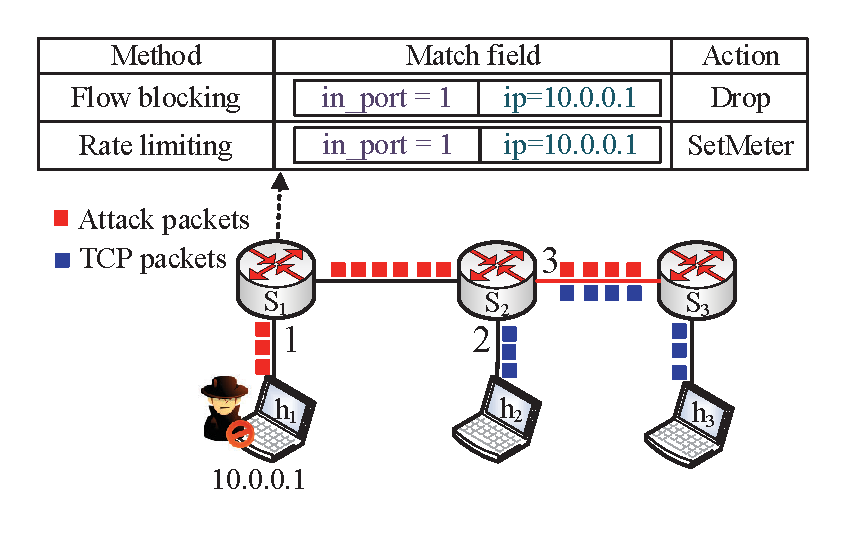
\includegraphics[scale=1]{defense}
    \caption{防御系统的一个例子,从$h_1$发送的LDos攻击流完全占用$S_2$与$S_3$之间连接的可用带宽。在$S_1$处,从$h_1$发送的LDoS攻击流被限制规则处理。}
    \label{fig:defense}
\end{figure}

图\ref{fig:defense}展示了攻击限制模块中限制规则的作用。在一个SDN网络中,攻击者$h_1$在交换机$S_1$的端口1处接入网络。合法用户$h_2$在在交换机$S_2$的端口2处接入网络。合法用户$h_3$在在交换机$S_3$的端口3处接入网络。假设$h_2$与$h_3$之间建立TCP连接,攻击者$h_1$想要完全占用$S_2$与$S_3$之间连接的可用带宽,并强迫$h_2$与$h_3$之间的TCP连接持续进入超时重传状态。在异常检测模块和攻击定位模块的帮助下,防御系统在$S_2$处识别了LDoS攻击,并且将攻击者$h_1$接入网络的端口1的信息通知给供给限制模块。攻击限制模块在入口交换机$S_1$处安装了相应的限制规则来阻塞或者限制$h_1$的流量。这样,攻击限制限制模块将完全消除LDoS攻击对于SDN网络的影响,$h_2$与$h_3$之间的TCP连接的吞吐量将会不在受到攻击者$h_1$的LDoS攻击的影响。

%Fig.~\ref{fig:mitigate} shows the mitigation method. The attacker $h_1$ accesses the network at port 1 and the legitimate user $h_2$ accesses the network at port 2 in the switch $S_1$. In addition, $h_2$ sends TCP packets to $h_3$. The attacker aims to overload the bandwidth of the link between $S_2$ and $S_3$ and thus to cause retransmission of the TCP flows between $h_2$ and $h_3$. The Locator module identifies the attack flow at $S_2$ and inform the Mitigator module on port 1. It blocks or limits the traffic of $h_1$ in the ingress switch $S_1$. Thus, the influence of the attack is eliminated and the TCP throughput of benign flows is not affected by the attack. 


由于LDoS攻击的特殊性,相应的限制规则是需要特别制定的。对于第一种方法,攻击限制模块想要阻塞LDoS攻击需要满足两个条件。首先安装在入口交换机的匹配LDoS攻击源的限制流表规则需要拥有最高的优先级,因为低优先级的限制规则会使一些攻击源的数据包避开限制流表规则而进入网络。因此,需要满足限制流表规则拥有所有流表规则中最高的优先级。其次,限制流表规则的指令必须是丢弃数据包,为了避免LDoS攻击的数据进入网络,最好的方案就是直接在交换机处丢弃攻击源的数据包。这样,在限制流表规则的作用下,LDoS攻击的数据包就无法进入网络,LDoS攻击将会被完全消除。但是,这也存在一定的风险,因为存在正常流量误判为攻击流的可能性,这些经过受影响端口的正常流也可能会受到影响。对于第二种方法,攻击限制模块使用了特制的Meter规则对LDoS攻击进行限制。对于限制LDoS攻击的Meter规则,burst\_size参数需要根据前面使用的$T_s$来特殊设置。攻击限制模块通过在入口交换机处安装特制的Meter规则,然后把与LDoS攻击流相关的流表规则与特制Meter规则绑定,就能达到限制LDoS突发速率的效果。

%For the first method, the flow rules that match the attack sources with the highest priority will be installed in the ingress switches. These rules block the attack flows at the ingress ports. The attack packets cannot be injected into the network anymore with the first method. Therefore, the influence of the attack will be eliminated. However, some benign traffic passing the blocked ingress ports may also be affected. In the second method, we leverage crafted meter rules, whose burst\_size is set based on $T_s$, for rate limitation. The Mitigator module assigns crafted meter rules to all the flow rules that match the attack traffic.

为了满足多种服务的需求,网络管理员根据不同的环境决定系统使用哪种方式限制LDoS攻击。一般情况下,阻塞LDoS攻击是限制LDoS攻击更好的方案。但是,管理者希望给所有主机保留一定的带宽以避免由于误判而对正常流的传输造成极大的影响。本系统默认的限制LDoS攻击的方法是阻塞LDoS流以保证SDN网络的安全性。

%To meet the various performance requirements, the network managers can determine which method is used in the system. In general, the first method is a better way to throttle the low-rate TCP attack. However, under the circumstances where the managers desire to reserve bandwidth for all the hosts, the second method is more suited to throttle the attack. The default method of our system is blocking the attack flows for the security of the network. 
\chapter{方案部署及其效果}
\label{cha:experiment}
本章的主要内容为部署防御方案并验证方案有效性。在真实SDN网络中部署防御方案之后,使用不同形式的LDoS攻击对方案进行测试,探测方案的有效性与开销。

\section{实验准备}
\label{chap5:setup}
本文在真实SDN网络中部署防御系统。防御系统使用的SDN控制器为Floodlight控制器。部署了防御系统的控制器被部署在一个服务器上,该服务器的配置为Intel Xeon Quad-Core CPU E5504和4GB的RAM。在系统中我们使用了OpenFlow商业硬件交换机(EdgeCore AS4610-54T)作为真实SDN网络使用的硬件交换机。硬件交换机的端口转发速率最高能够可达到1Gbps,本文将最大转发速率标记为$R_m$。为了验证系统有效性,本文使用C代码生成不同$T$与$L$的LDoS攻击。并且使用Python代码完成分布式LDoS攻击的部署。

图\ref{fig:topology}展示了实验使用的SDN网络拓扑图。它有7个主机和3个OpenFlow硬件交换机组成。其中2个主机为攻击主机,5个主机为正常的主机。在实验中,$h_1$发送正常流量作为背景流量并由$h_5$接收,$h_3$与$h_6$之间建立TCP连接。$h_2$和$h_4$被设置为LDoS攻击的发送端,由$h_7$接收他们发送的LDoS攻击流量。对于攻击者$h_2$和$h_4$的不同配置可以得到单一攻击源的LDoS攻击,也可以得到分布式LDoS攻击。

%对于这个网络,LDoS攻击流的目的是完全占用$S_2$与$S_3$之间连接的带宽致使$S_2$的队列被拥塞造成$h_1$

\begin{figure}
    \centering
    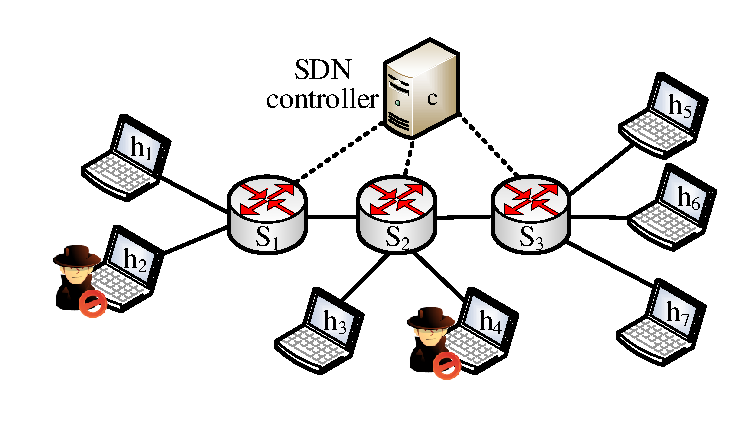
\includegraphics[scale=1]{topology}
    \caption{实验使用拓扑图}
    \label{fig:topology}
\end{figure}


\section{基于带宽保障的方案}

\section{基于动态周期性检测的防御方案}
\label{chap5:expperioddetection}
在系统部署了基于动态周期性检测的方案之后,本文通过对检测精确度和方案的开销对方案进行全方位的讨论和分析,对方案的有效性进行评价。对方案的评估包括一个主机完成LDoS攻击和两个主机完成LDoS攻击两种形式。

\subsection{精确度分析}
\label{chap5:accuracy}
这个部分主要分析基于动态周期性检测的防御方案的各个模块的准确性和稳定性。首先,本文对异常检测模块成功检测到端口异常的成功率做实验进行分析。然后,本文计算了攻击定位模块推断出的LDoS攻击周期与真正的LDoS周期之间的误差。接下来,本文通过实验获得了经过受影响端口与经过端口流量的平均欧式距离的概率密度函数(Probability Density Function,PDF),并在此基础上,找到了用于判断攻击流的阈值。最后,本文探索了平均欧式方法判断攻击流的准确度。

异常检测模块在异常端口处检测到可能的LDoS攻击时才会激活攻击定位模块对异常端口进行进一步的分析,因此,该模块在LDoS攻击存在的情况下检测到端口吞吐量异常的成功率直接关键到LDoS攻击能否被系统检测,因此,本文对异常检测模块的参数$\alpha$和$M$进行了探讨。

% alpha,M两个参数进行分析讨论,出图,(1-2页)

% alpha和LDoS识别率,M作为稳定参数,多次取值,准确识别LDoS的图

% alpha和误判率,M作为稳定参数,多次取值,正常流判断为LDoS流


攻击定位模块的第一步是对序列进行二值化,本文将阈值$\beta$设为0.8。接下来,本文通过对异常端口的计数器获取的数据推测LDoS攻击的周期。在获得二值化序列之后,本文对该序列进行周期性的推测。如果在异常的端口处存在LDoS攻击流,则推断出的序列周期将会是一个正数。但是,如果端口不存在LDoS攻击流,则推断出的序列周期将会为0。为了获得攻击定位模块推断的周期准确度,本文比较通过序列推断出的周期与LDoS攻击流的真实周期,得到了推断的周期误差。

\begin{figure}
    \centering
    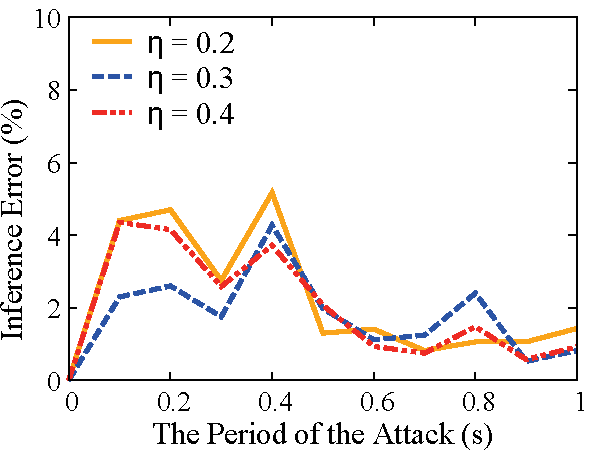
\includegraphics[scale=1.0]{period}
    \caption{推断误差}
    \label{fig:period}
\end{figure}

图\ref{fig:period}展示了不同LDoS攻击的周期下,攻击定位模块推断的周期与真实LDoS攻击的周期的相对误差。此处使用算法\ref{alg:port_locate}来预测LDoS攻击的周期。实验中,我们将LDoS攻击的突发速率$R$置为1Gbps。对于算法的参数,考虑系统的带宽和识别率保证,本文设定$T_e$为0.005,$T_i$为0.64,$\epsilon$ = 0.01。为了查看算法对LDoS攻击周期的适应性,在LDoS攻击的周期从0.1上升至1s的情况下,使用攻击检测模块对不同$\eta$值的LDoS攻击的周期进行预测。除此之外,还使用洪泛攻击测试算法。每次使用5秒获取端口的数据进行测试。实验的结果表示,攻击检测模块能够确认异常端口上的LDoS攻击,同时,推测出来的周期也存在一定的误差,但是,推断出的相对误差最多不超过6\%。LDoS攻击不存在(洪泛攻击)的情况下,由于洪泛攻击没有周期,而推断出的周期为0,因此,在0点处,误差为0。在大多数情况下,在LDoS攻击的周期值比较小的时候,相对误差会比较大。攻击检测模块的绝对误差在0至30毫秒之间,随着算法的周期不断变大,攻击检测模块的相对误差也相应的减小。通过这次实验也获得了相应的$T_s$。攻击定位模块在确认了LDoS攻击在异常端口存在之后,使用了$T_s$作为采样间隔获取流表规则上的计数器数据用以对识别攻击流。

在确认端口受LDoS攻击影响之后,控制器以$T_s$的采样间隔同时获取受影响端口序列与经过该端口的流的信息,在通过二值化之后对二值化流量做进一步分析。在LDoS攻击的$T$设为1秒,$L$设为0.2秒的时候,控制器以$T_s$为0.2s获取流表规则计数器上的数据,则可以获得受影响端口、正常数据流和LDoS攻击流的吞吐量二值化序列。如图\ref{fig:binary-sequence}所示,三者的吞吐量二值化序列的形状是完全不同的,受影响端口的二值化序列的形状与LDoS攻击流的二值化序列更加相近,而背景流量的形状则与受影响端口的二值化序列不相似。在LDoS突发出现的时候,即图中LDoS攻击的二值化吞吐量值为1的时候,受影响端口的二值化吞吐量也为1,此时,背景流量的二值化吞吐量为0,因为,在LDoS攻击的突发时间里的情况下,交换机转发的背景流量低于没有LDoS攻击时的最高速率,在二值化的时候把该时刻的值置为0。在LDoS攻击存在的情况下,受影响端口统计的吞吐量序列最大值$S_m$即为$R_m$,因此,受影响端口统计的吞吐量序列中流量的速率在LDoS攻击不存在的情况下基本低于$\beta * S_m$。受影响端口在LDoS攻击不存在的情况下的二值化吞吐量基本为0。从此图中也可以,使用平均欧式距离区分LDoS攻击流与背景流是可行的。



\begin{figure}
    \centering
    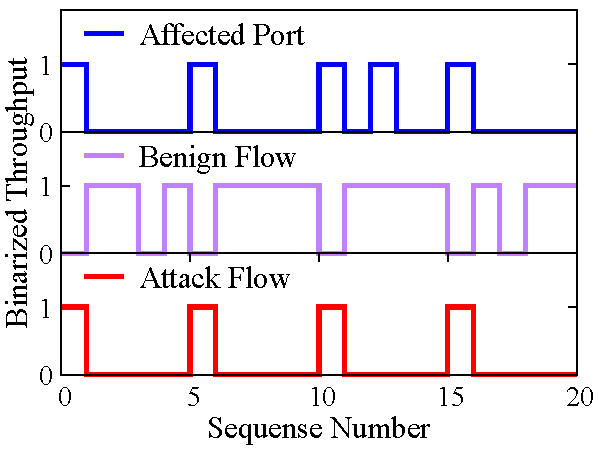
\includegraphics[scale=1.3]{binary-sequence}
    \caption{二值化吞吐量序列}
    \label{fig:binary-sequence}
\end{figure}



为了获得合适的阈值$\gamma$来识别攻击流,受影响端口的二值化序列与经过该端口的数据流的平均欧式距离的概率密度函数是必须的,但是一个攻击源与多个攻击源的情况不同,因此,需要多次试验来分析不同的情况下。LDoS攻击流平均欧氏距离与正常数据流的平均欧氏距离是完全不同的。在经过了二值化之后,LDoS攻击流的二值化序列与受影响端口统计的二值化序列的平均欧式距离比正常流量小很多,因此,找到合适的阈值$\gamma$,就可以识别攻击流。首先,考虑验证系统对于大部分情况的适应性,只用一个固定的$T$是不足够的,所以,LDoS攻击的$T$随机从0.8至1.5之前取值,因为LDoS攻击的$T$取值过大会是TCP流无法进入超时重传状态。接下来,考虑到$L$的取值不应过小或者过大,设置LDoS攻击的突发长度$L$从0.1至0.4之间随机取值。如果$L$太小,则无法造成TCP流丢包,则无法达到LDoS攻击的效果。但是,如果$L$的取值过大,则平均速率会很高,容易被洪泛服务拒绝攻击的检测方式检测到。最后,考虑交换机最大转发速率为1Gbps,所以,LDoS攻击的突发速率$R$设为1Gbps已经是能够达到的最大速率了,如果突发速率更高则可能造成LDoS攻击自身丢包过多,反而容易被检测到。考虑到需要有背景流量作为良性的流量干扰防御系统以验证攻击定位模块的有效性,$h_1$生成了100条良性流作为背景流量发送给$h_5$。

本文先分析一个攻击源生成LDoS攻击的情况。以$h_2$作为攻击源发送LDoS攻击流,$h_4$不发送攻击流量。经过多次试验,获得图\ref{fig:PDF-single}作为单攻击源的概率密度函数。可以看到,LDoS攻击流的二值化序列与受影响端口的二值化序列的平均欧式距离的主要分布在0.2与0.4之间,平均值为0.3。而正常流的二值化序列与受影响端口的二值化序列的平均欧式距离的主要分布在0.44至0.84之间,平均值为0.64。绝大部分情况下,LDoS攻击流的二值化序列与受影响端口的二值化序列的平均欧式距离比正常流的二值化序列与受影响端口的二值化序列的平均欧式距离小。因为在LDoS攻击突发存在的情况下,端口转发的主要流量为LDoS攻击。而没有LDoS攻击攻击存在的时候,正常流公平竞争带宽,因此,速率更高,在突发不存在的时候,二值化吞吐量值为1,受影响端口的二值化序列为0,刚好相反,因此平均欧式距离更大。从图\ref{fig:PDF-single}中可以看到一个清晰的区分点,即$MED$为0.42。该点可以作为识别单攻击源中LDoS攻击流的阈值。

\begin{figure}
    \begin{minipage}[t]{0.49\linewidth}
        \centering
        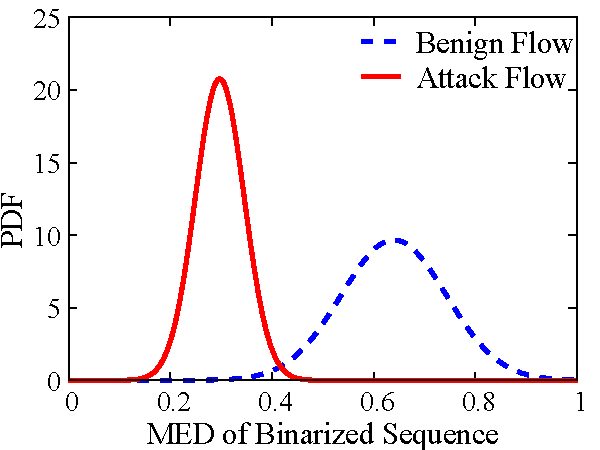
\includegraphics[scale=0.7]{distribution}
        \caption{\small{单攻击源的平均欧式距离的PDF}}
        \label{fig:PDF-single}
    \end{minipage}
    \begin{minipage}[t]{0.49\linewidth}
        \centering
        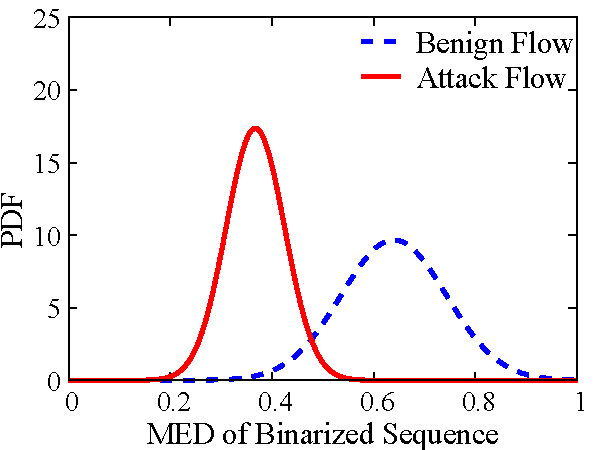
\includegraphics[scale=0.7]{distribution1}
        \caption{\small{分布式方案一平均欧式距离的PDF}}
        \label{fig:PDF-2h-mod1}
    \end{minipage}

    \begin{minipage}[t]{0.49\linewidth}
        \centering
        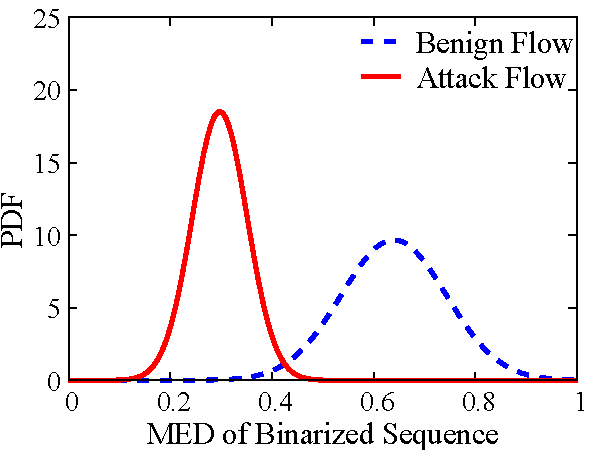
\includegraphics[scale=0.7]{distribution2}
        \caption{\small{分布式方案二平均欧式距离的PDF}}
        \label{fig:PDF-2h-mod2}
    \end{minipage}
        \begin{minipage}[t]{0.49\linewidth}
        \centering
        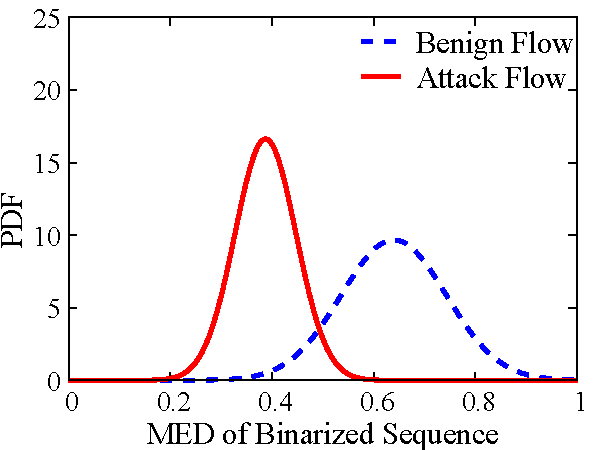
\includegraphics[scale=0.7]{distribution3}
        \caption{\small{分布式方案三平均欧式距离的PDF}}
        \label{fig:PDF-2h-mod3}
    \end{minipage}
\end{figure}

在获得单攻击源的平均欧式距离的概率分布函数之后,可以确认使用平均欧氏距离的方法确实可以区分攻击流与正常流。接下来,对多攻击源分布式LDoS攻击进行区分,因此,以$h_2$和$h_4$同时作为攻击源发送LDoS攻击流,分布式LDoS攻击的三种方案产生流量,获得相应的平均欧式距离的概率密度函数。两主机以分布式方案一的方式产生LDoS攻击的流量,获得图\ref{fig:PDF-2h-mod1}。从图中可看出,与单攻击源不同,LDoS攻击流的二值化序列与受影响端口的二值化序列的平均欧式距离的主要分布发生了变化,主要分布在0.24至0.48,平均值为0.36,而正常流的二值化序列与受影响端口的二值化序列的平均欧式距离的主要分布在0.45至0.85之间,平均值为0.65。以方案一平均欧式距离的分布函数平均值变大,因为在受影响端口处统计的突发包括了两个主机的突发流量,而使用流表规则统计的数据只包含一个流的数据,因此,计算出的平均欧式距离统计的平均值相较于单攻击源的平均欧式距离统计的平均值更大。因此,对于方案一而言,最佳的区分点为0.47。

当两个主机以分布式方案二的方式产生LDoS攻击的流量,获得图\ref{fig:PDF-2h-mod2}。从图中可看出,LDoS攻击流的二值化序列与受影响端口的二值化序列的平均欧式距离的主要分布与

% \begin{figure}
%     \centering
%     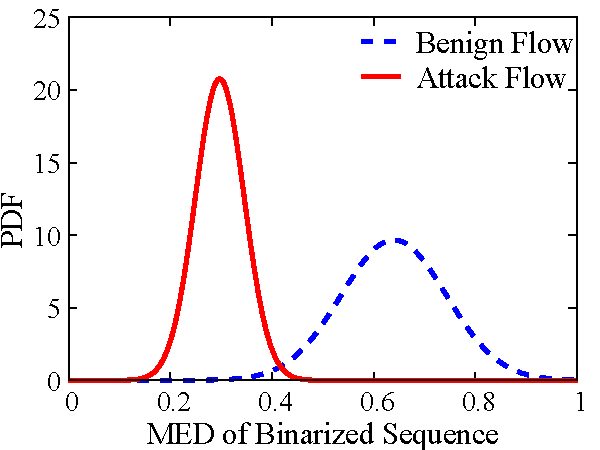
\includegraphics[scale=0.6]{distribution}
%     \caption{平均欧式距离的概率密度函数}
%     \label{fig:PDFofMED}
% \end{figure}



%二值化后数据对比










%%% 其它部分
\backmatter

%% 本科生要这几个索引,研究生不要。选择性留下。
% 插图索引
\listoffigures
% 表格索引
\listoftables
% 公式索引
\listofequations


%% 参考文献
% 注意:至少需要引用一篇参考文献,否则下面两行可能引起编译错误。
% 如果不需要参考文献,请将下面两行删除或注释掉。
\bibliographystyle{thuthesis-numeric}      % 顺序编码制
% \bibliographystyle{thuthesis-author-year}  % 著者-出版年制
% \bibliographystyle{thuthesis-bachelor}     % 本科生参考文献的著录格式
\bibliography{ref/refs}


%% 致谢
% 如果使用声明扫描页,将可选参数指定为扫描后的 PDF 文件名,例如:
% \begin{acknowledgement}[scan-statement.pdf]
\begin{acknowledgement}
  首先,衷心感谢我的导师徐明伟教授,徐老师平易近人,总能给人温暖的感觉;在科研上总能够有很独到的见解,可以指明前进的方向,让人心生敬佩。徐老师在我的科研和生活中帮助极大,给我树立了很好的学习的榜样,让我有了不断前进的动力。能够成为徐老师的学生,是人生中最开心的一件事。

  其次,我也要向李琦老师和曹家浩师兄表示感谢。他们在我硕士期间对本人悉心指导,经常与我讨论科研,让我能够快速入门,并掌握一些方法。在与他们的交流中,我逐步提升自己,感受到自己的成长。同时也感谢实验室的同学一直以来的支持,尤其是耿男同学,在我迷茫的时候,总能陪伴并鼓励我,让我走出了困境。

  特别地,我要感谢一直以来和我相互帮助的何阳同学,他给了我面对绝望的勇气和永不言弃的毅力,期待以后共同的成长。感谢教会我思考方式的冯伟伦师兄,在与他生活学习的时间里,我逐渐学习到探索本质的方法。

  最后,我想感谢我的父母一直对我无条件的支持和帮助,感谢netlab实验室给了我学习和科研的条件,感谢学校给了我终生难忘的美好时光。

  本课题承蒙国家自然科学基金资助,特此致谢。

  感谢 \LaTeX 和 \thuthesis\cite{thuthesis},帮我节省了不少时间。
\end{acknowledgement}


%% 附录
\begin{appendix}
\input{data/appendix01}
\end{appendix}

%% 个人简历
\begin{resume}

  \resumeitem{个人简历}

  1994 年 8 月 18 日出生于 广西 省 永福 县。

  2012 年 9 月考入 北京邮电 大学 信息与通信工程 学院 信息 专业,2016 年 7 月本科毕业并获得 工学 学士学位。

  2016 年 9 月免试进入 清华 大学 计算机科学与技术 系攻读 硕士 学位至今。

  \researchitem{发表的学术论文} % 发表的和录用的合在一起

  % 1. 已经刊载的学术论文(本人是第一作者,或者导师为第一作者本人是第二作者)
  % \begin{publications}
  %   \item Yang Y, Ren T L, Zhang L T, et al. Miniature microphone with silicon-
  %     based ferroelectric thin films. Integrated Ferroelectrics, 2003,
  %     52:229-235. (SCI 收录, 检索号:758FZ.)
  %   \item 杨轶, 张宁欣, 任天令, 等. 硅基铁电微声学器件中薄膜残余应力的研究. 中国机
  %     械工程, 2005, 16(14):1289-1291. (EI 收录, 检索号:0534931 2907.)
  %   \item 杨轶, 张宁欣, 任天令, 等. 集成铁电器件中的关键工艺研究. 仪器仪表学报,
  %     2003, 24(S4):192-193. (EI 源刊.)
  % \end{publications}

  % 2. 尚未刊载,但已经接到正式录用函的学术论文(本人为第一作者,或者
  %    导师为第一作者本人是第二作者)。
  \begin{publications}[before=\publicationskip,after=\publicationskip]
    % \item Yang Y, Ren T L, Zhu Y P, et al. PMUTs for handwriting recognition. In
    %   press. (已被 Integrated Ferroelectrics 录用. SCI 源刊.)

    \item Renjie Xie, Mingwei Xu, Jiahao Cao, Qi Li. “ SoftGuard: Defend against the Low-Rate TCP Attack in SDN. ” 2019 IEEE International Conference on Communications (ICC): Communication and Information Systems Security Symposium (IEEE ICC'19 - CISS Symposium), Shanghai, P.R. China, May 2019. (已被ICC录用,CCF-C)

    
    
  \end{publications}

  % 3. 其他学术论文。可列出除上述两种情况以外的其他学术论文,但必须是
  %    已经刊载或者收到正式录用函的论文。
  \begin{publications}
    \item Jiahao Cao, Qi Li, Renjie Xie, et al. “The CrossPath Attack: Disrupting the SDN Control Channel via Shared Links,” In Proc. of the 28th USENIX Security Symposium (USENIX Security), Santa Clara, CA, August 2019(已被Usenix Security 录用, CCF-A)
  \end{publications}

  % \researchitem{研究成果} % 有就写,没有就删除
  % \begin{achievements}
  %   \item 任天令, 杨轶, 朱一平, 等. 硅基铁电微声学传感器畴极化区域控制和电极连接的
  %     方法: 中国, CN1602118A. (中国专利公开号)
  %   \item Ren T L, Yang Y, Zhu Y P, et al. Piezoelectric micro acoustic sensor
  %     based on ferroelectric materials: USA, No.11/215, 102. (美国发明专利申请号)
  % \end{achievements}

\end{resume}


%% 本科生进行格式审查是需要下面这个表格,答辩可能不需要。选择性留下。
% 综合论文训练记录表
\includepdf[pages=-]{scan-record.pdf}
\end{document}
